%%%%%%%% ICML 2026 EXAMPLE LATEX SUBMISSION FILE %%%%%%%%%%%%%%%%%

\documentclass{article}

% Recommended, but optional, packages for figures and better typesetting:
\usepackage{microtype}
\usepackage{graphicx}
\usepackage{subcaption}
\usepackage{booktabs} % for professional tables

% hyperref makes hyperlinks in the resulting PDF.
% If your build breaks (sometimes temporarily if a hyperlink spans a page)
% please comment out the following usepackage line and replace
% \usepackage{icml2026} with \usepackage[nohyperref]{icml2026} above.
\usepackage{hyperref}


% Attempt to make hyperref and algorithmic work together better:
\newcommand{\theHalgorithm}{\arabic{algorithm}}

% Use the following line for the initial blind version submitted for review:
\usepackage{icml2026}

% For preprint, use
% \usepackage[preprint]{icml2026}

% If accepted, instead use the following line for the camera-ready submission:
% \usepackage[accepted]{icml2026}

%%%%% NEW MATH DEFINITIONS %%%%%

\usepackage{amsmath,amsfonts,bm,}

% Our own additions
\newcommand{\inner}[2]{\left\langle #1, #2 \right\rangle}
\newcommand{\vttheta}{{\bm{\theta}}}
\newcommand{\vta}{{\bm{a}}}
\newcommand{\vtaj}{{\bm{a}^j}}
\newcommand{\vtb}{{\bm{b}}}
\newcommand{\vtz}{{\bm{z}}}
\newcommand{\vtx}{{\bm{x}}}
\newcommand{\vty}{{\bm{y}}}
\newcommand{\vtv}{{\bm{v}}}
\newcommand{\vtzp}{{\bm{z}'}}
\newcommand{\vtsj}{{\bm{s}^j}}
\newcommand{\vtsji}{{\bm{s}^j_k}}
\newcommand{\vtsl}{{\bm{s}^\ell}}
\newcommand{\vts}{{\bm{s}}}
%\usepackage{dsfont}
\usepackage{physics}

% Mark sections of captions for referring to divisions of figures
\newcommand{\figleft}{{\em (Left)}}
\newcommand{\figcenter}{{\em (Center)}}
\newcommand{\figright}{{\em (Right)}}
\newcommand{\figtop}{{\em (Top)}}
\newcommand{\figbottom}{{\em (Bottom)}}
\newcommand{\captiona}{{\em (a)}}
\newcommand{\captionb}{{\em (b)}}
\newcommand{\captionc}{{\em (c)}}
\newcommand{\captiond}{{\em (d)}}

% Highlight a newly defined term
\newcommand{\newterm}[1]{{\bf #1}}


% Figure reference, lower-case.
\def\figref#1{figure~\ref{#1}}
% Figure reference, capital. For start of sentence
\def\Figref#1{Figure~\ref{#1}}
\def\twofigref#1#2{figures \ref{#1} and \ref{#2}}
\def\quadfigref#1#2#3#4{figures \ref{#1}, \ref{#2}, \ref{#3} and \ref{#4}}
% Section reference, lower-case.
\def\secref#1{section~\ref{#1}}
% Section reference, capital.
\def\Secref#1{Section~\ref{#1}}
% Reference to two sections.
\def\twosecrefs#1#2{sections \ref{#1} and \ref{#2}}
% Reference to three sections.
\def\secrefs#1#2#3{sections \ref{#1}, \ref{#2} and \ref{#3}}
% Reference to an equation, lower-case.
\def\eqref#1{equation~\ref{#1}}
% Reference to an equation, upper case
\def\Eqref#1{Equation~\ref{#1}}
% A raw reference to an equation---avoid using if possible
\def\plaineqref#1{\ref{#1}}
% Reference to a chapter, lower-case.
\def\chapref#1{chapter~\ref{#1}}
% Reference to an equation, upper case.
\def\Chapref#1{Chapter~\ref{#1}}
% Reference to a range of chapters
\def\rangechapref#1#2{chapters\ref{#1}--\ref{#2}}
% Reference to an algorithm, lower-case.
\def\algref#1{algorithm~\ref{#1}}
% Reference to an algorithm, upper case.
\def\Algref#1{Algorithm~\ref{#1}}
\def\twoalgref#1#2{algorithms \ref{#1} and \ref{#2}}
\def\Twoalgref#1#2{Algorithms \ref{#1} and \ref{#2}}
% Reference to a part, lower case
\def\partref#1{part~\ref{#1}}
% Reference to a part, upper case
\def\Partref#1{Part~\ref{#1}}
\def\twopartref#1#2{parts \ref{#1} and \ref{#2}}

\def\ceil#1{\lceil #1 \rceil}
\def\floor#1{\lfloor #1 \rfloor}
\def\1{\bm{1}}
\newcommand{\train}{\mathcal{D}}
\newcommand{\valid}{\mathcal{D_{\mathrm{valid}}}}
\newcommand{\test}{\mathcal{D_{\mathrm{test}}}}

\def\eps{{\epsilon}}


% Random variables
\def\reta{{\textnormal{$\eta$}}}
\def\ra{{\textnormal{a}}}
\def\rb{{\textnormal{b}}}
\def\rc{{\textnormal{c}}}
\def\rd{{\textnormal{d}}}
\def\re{{\textnormal{e}}}
\def\rf{{\textnormal{f}}}
\def\rg{{\textnormal{g}}}
\def\rh{{\textnormal{h}}}
\def\ri{{\textnormal{i}}}
\def\rj{{\textnormal{j}}}
\def\rk{{\textnormal{k}}}
\def\rl{{\textnormal{l}}}
% rm is already a command, just don't name any random variables m
\def\rn{{\textnormal{n}}}
\def\ro{{\textnormal{o}}}
\def\rp{{\textnormal{p}}}
\def\rq{{\textnormal{q}}}
\def\rr{{\textnormal{r}}}
\def\rs{{\textnormal{s}}}
\def\rt{{\textnormal{t}}}
\def\ru{{\textnormal{u}}}
\def\rv{{\textnormal{v}}}
\def\rw{{\textnormal{w}}}
\def\rx{{\textnormal{x}}}
\def\ry{{\textnormal{y}}}
\def\rz{{\textnormal{z}}}

% Random vectors
\def\rvepsilon{{\mathbf{\epsilon}}}
\def\rvtheta{{\mathbf{\theta}}}
\def\rva{{\mathbf{a}}}
\def\rvb{{\mathbf{b}}}
\def\rvc{{\mathbf{c}}}
\def\rvd{{\mathbf{d}}}
\def\rve{{\mathbf{e}}}
\def\rvf{{\mathbf{f}}}
\def\rvg{{\mathbf{g}}}
\def\rvh{{\mathbf{h}}}
\def\rvu{{\mathbf{i}}}
\def\rvj{{\mathbf{j}}}
\def\rvk{{\mathbf{k}}}
\def\rvl{{\mathbf{l}}}
\def\rvm{{\mathbf{m}}}
\def\rvn{{\mathbf{n}}}
\def\rvo{{\mathbf{o}}}
\def\rvp{{\mathbf{p}}}
\def\rvq{{\mathbf{q}}}
\def\rvr{{\mathbf{r}}}
\def\rvs{{\mathbf{s}}}
\def\rvt{{\mathbf{t}}}
\def\rvu{{\mathbf{u}}}
\def\rvv{{\mathbf{v}}}
\def\rvw{{\mathbf{w}}}
\def\rvx{{\mathbf{x}}}
\def\rvy{{\mathbf{y}}}
\def\rvz{{\mathbf{z}}}

% Elements of random vectors
\def\erva{{\textnormal{a}}}
\def\ervb{{\textnormal{b}}}
\def\ervc{{\textnormal{c}}}
\def\ervd{{\textnormal{d}}}
\def\erve{{\textnormal{e}}}
\def\ervf{{\textnormal{f}}}
\def\ervg{{\textnormal{g}}}
\def\ervh{{\textnormal{h}}}
\def\ervi{{\textnormal{i}}}
\def\ervj{{\textnormal{j}}}
\def\ervk{{\textnormal{k}}}
\def\ervl{{\textnormal{l}}}
\def\ervm{{\textnormal{m}}}
\def\ervn{{\textnormal{n}}}
\def\ervo{{\textnormal{o}}}
\def\ervp{{\textnormal{p}}}
\def\ervq{{\textnormal{q}}}
\def\ervr{{\textnormal{r}}}
\def\ervs{{\textnormal{s}}}
\def\ervt{{\textnormal{t}}}
\def\ervu{{\textnormal{u}}}
\def\ervv{{\textnormal{v}}}
\def\ervw{{\textnormal{w}}}
\def\ervx{{\textnormal{x}}}
\def\ervy{{\textnormal{y}}}
\def\ervz{{\textnormal{z}}}

% Random matrices
\def\rmA{{\mathbf{A}}}
\def\rmB{{\mathbf{B}}}
\def\rmC{{\mathbf{C}}}
\def\rmD{{\mathbf{D}}}
\def\rmE{{\mathbf{E}}}
\def\rmF{{\mathbf{F}}}
\def\rmG{{\mathbf{G}}}
\def\rmH{{\mathbf{H}}}
\def\rmI{{\mathbf{I}}}
\def\rmJ{{\mathbf{J}}}
\def\rmK{{\mathbf{K}}}
\def\rmL{{\mathbf{L}}}
\def\rmM{{\mathbf{M}}}
\def\rmN{{\mathbf{N}}}
\def\rmO{{\mathbf{O}}}
\def\rmP{{\mathbf{P}}}
\def\rmQ{{\mathbf{Q}}}
\def\rmR{{\mathbf{R}}}
\def\rmS{{\mathbf{S}}}
\def\rmT{{\mathbf{T}}}
\def\rmU{{\mathbf{U}}}
\def\rmV{{\mathbf{V}}}
\def\rmW{{\mathbf{W}}}
\def\rmX{{\mathbf{X}}}
\def\rmY{{\mathbf{Y}}}
\def\rmZ{{\mathbf{Z}}}

% Elements of random matrices
\def\ermA{{\textnormal{A}}}
\def\ermB{{\textnormal{B}}}
\def\ermC{{\textnormal{C}}}
\def\ermD{{\textnormal{D}}}
\def\ermE{{\textnormal{E}}}
\def\ermF{{\textnormal{F}}}
\def\ermG{{\textnormal{G}}}
\def\ermH{{\textnormal{H}}}
\def\ermI{{\textnormal{I}}}
\def\ermJ{{\textnormal{J}}}
\def\ermK{{\textnormal{K}}}
\def\ermL{{\textnormal{L}}}
\def\ermM{{\textnormal{M}}}
\def\ermN{{\textnormal{N}}}
\def\ermO{{\textnormal{O}}}
\def\ermP{{\textnormal{P}}}
\def\ermQ{{\textnormal{Q}}}
\def\ermR{{\textnormal{R}}}
\def\ermS{{\textnormal{S}}}
\def\ermT{{\textnormal{T}}}
\def\ermU{{\textnormal{U}}}
\def\ermV{{\textnormal{V}}}
\def\ermW{{\textnormal{W}}}
\def\ermX{{\textnormal{X}}}
\def\ermY{{\textnormal{Y}}}
\def\ermZ{{\textnormal{Z}}}

% Vectors
\def\vzero{{\bm{0}}}
\def\vone{{\bm{1}}}
\def\vmu{{\bm{\mu}}}
\def\vtheta{{\bm{\theta}}}
\def\va{{\bm{a}}}
\def\vb{{\bm{b}}}
\def\vc{{\bm{c}}}
\def\vd{{\bm{d}}}
\def\ve{{\bm{e}}}
\def\vf{{\bm{f}}}
\def\vg{{\bm{g}}}
\def\vh{{\bm{h}}}
\def\vi{{\bm{i}}}
\def\vj{{\bm{j}}}
\def\vk{{\bm{k}}}
\def\vl{{\bm{l}}}
\def\vm{{\bm{m}}}
\def\vn{{\bm{n}}}
\def\vo{{\bm{o}}}
\def\vp{{\bm{p}}}
\def\vq{{\bm{q}}}
\def\vr{{\bm{r}}}
\def\vs{{\bm{s}}}
\def\vt{{\bm{t}}}
\def\vu{{\bm{u}}}
\def\vv{{\bm{v}}}
\def\vw{{\bm{w}}}
\def\vx{{\bm{x}}}
\def\vy{{\bm{y}}}
\def\vz{{\bm{z}}}

% Elements of vectors
\def\evalpha{{\alpha}}
\def\evbeta{{\beta}}
\def\evepsilon{{\epsilon}}
\def\evlambda{{\lambda}}
\def\evomega{{\omega}}
\def\evmu{{\mu}}
\def\evpsi{{\psi}}
\def\evsigma{{\sigma}}
\def\evtheta{{\theta}}
\def\eva{{a}}
\def\evb{{b}}
\def\evc{{c}}
\def\evd{{d}}
\def\eve{{e}}
\def\evf{{f}}
\def\evg{{g}}
\def\evh{{h}}
\def\evi{{i}}
\def\evj{{j}}
\def\evk{{k}}
\def\evl{{l}}
\def\evm{{m}}
\def\evn{{n}}
\def\evo{{o}}
\def\evp{{p}}
\def\evq{{q}}
\def\evr{{r}}
\def\evs{{s}}
\def\evt{{t}}
\def\evu{{u}}
\def\evv{{v}}
\def\evw{{w}}
\def\evx{{x}}
\def\evy{{y}}
\def\evz{{z}}

% Matrix
\def\mA{{\bm{A}}}
\def\mB{{\bm{B}}}
\def\mC{{\bm{C}}}
\def\mD{{\bm{D}}}
\def\mE{{\bm{E}}}
\def\mF{{\bm{F}}}
\def\mG{{\bm{G}}}
\def\mH{{\bm{H}}}
\def\mI{{\bm{I}}}
\def\mJ{{\bm{J}}}
\def\mK{{\bm{K}}}
\def\mL{{\bm{L}}}
\def\mM{{\bm{M}}}
\def\mN{{\bm{N}}}
\def\mO{{\bm{O}}}
\def\mP{{\bm{P}}}
\def\mQ{{\bm{Q}}}
\def\mR{{\bm{R}}}
\def\mS{{\bm{S}}}
\def\mT{{\bm{T}}}
\def\mU{{\bm{U}}}
\def\mV{{\bm{V}}}
\def\mW{{\bm{W}}}
\def\mX{{\bm{X}}}
\def\mY{{\bm{Y}}}
\def\mZ{{\bm{Z}}}
\def\mBeta{{\bm{\beta}}}
\def\mPhi{{\bm{\Phi}}}
\def\mLambda{{\bm{\Lambda}}}
\def\mSigma{{\bm{\Sigma}}}

% Tensor
\DeclareMathAlphabet{\mathsfit}{\encodingdefault}{\sfdefault}{m}{sl}
\SetMathAlphabet{\mathsfit}{bold}{\encodingdefault}{\sfdefault}{bx}{n}
\newcommand{\tens}[1]{\bm{\mathsfit{#1}}}
\def\tA{{\tens{A}}}
\def\tB{{\tens{B}}}
\def\tC{{\tens{C}}}
\def\tD{{\tens{D}}}
\def\tE{{\tens{E}}}
\def\tF{{\tens{F}}}
\def\tG{{\tens{G}}}
\def\tH{{\tens{H}}}
\def\tI{{\tens{I}}}
\def\tJ{{\tens{J}}}
\def\tK{{\tens{K}}}
\def\tL{{\tens{L}}}
\def\tM{{\tens{M}}}
\def\tN{{\tens{N}}}
\def\tO{{\tens{O}}}
\def\tP{{\tens{P}}}
\def\tQ{{\tens{Q}}}
\def\tR{{\tens{R}}}
\def\tS{{\tens{S}}}
\def\tT{{\tens{T}}}
\def\tU{{\tens{U}}}
\def\tV{{\tens{V}}}
\def\tW{{\tens{W}}}
\def\tX{{\tens{X}}}
\def\tY{{\tens{Y}}}
\def\tZ{{\tens{Z}}}


% Graph
\def\gA{{\mathcal{A}}}
\def\gB{{\mathcal{B}}}
\def\gC{{\mathcal{C}}}
\def\gD{{\mathcal{D}}}
\def\gE{{\mathcal{E}}}
\def\gF{{\mathcal{F}}}
\def\gG{{\mathcal{G}}}
\def\gH{{\mathcal{H}}}
\def\gI{{\mathcal{I}}}
\def\gJ{{\mathcal{J}}}
\def\gK{{\mathcal{K}}}
\def\gL{{\mathcal{L}}}
\def\gM{{\mathcal{M}}}
\def\gN{{\mathcal{N}}}
\def\gO{{\mathcal{O}}}
\def\gP{{\mathcal{P}}}
\def\gQ{{\mathcal{Q}}}
\def\gR{{\mathcal{R}}}
\def\gS{{\mathcal{S}}}
\def\gT{{\mathcal{T}}}
\def\gU{{\mathcal{U}}}
\def\gV{{\mathcal{V}}}
\def\gW{{\mathcal{W}}}
\def\gX{{\mathcal{X}}}
\def\gY{{\mathcal{Y}}}
\def\gZ{{\mathcal{Z}}}

% Sets
\def\sA{{\mathbb{A}}}
\def\sB{{\mathbb{B}}}
\def\sC{{\mathbb{C}}}
\def\sD{{\mathbb{D}}}
% Don't use a set called E, because this would be the same as our symbol
% for expectation.
\def\sF{{\mathbb{F}}}
\def\sG{{\mathbb{G}}}
\def\sH{{\mathbb{H}}}
\def\sI{{\mathbb{I}}}
\def\sJ{{\mathbb{J}}}
\def\sK{{\mathbb{K}}}
\def\sL{{\mathbb{L}}}
\def\sM{{\mathbb{M}}}
\def\sN{{\mathbb{N}}}
\def\sO{{\mathbb{O}}}
\def\sP{{\mathbb{P}}}
\def\sQ{{\mathbb{Q}}}
\def\sR{{\mathbb{R}}}
\def\sS{{\mathbb{S}}}
\def\sT{{\mathbb{T}}}
\def\sU{{\mathbb{U}}}
\def\sV{{\mathbb{V}}}
\def\sW{{\mathbb{W}}}
\def\sX{{\mathbb{X}}}
\def\sY{{\mathbb{Y}}}
\def\sZ{{\mathbb{Z}}}

% Entries of a matrix
\def\emLambda{{\Lambda}}
\def\emA{{A}}
\def\emB{{B}}
\def\emC{{C}}
\def\emD{{D}}
\def\emE{{E}}
\def\emF{{F}}
\def\emG{{G}}
\def\emH{{H}}
\def\emI{{I}}
\def\emJ{{J}}
\def\emK{{K}}
\def\emL{{L}}
\def\emM{{M}}
\def\emN{{N}}
\def\emO{{O}}
\def\emP{{P}}
\def\emQ{{Q}}
\def\emR{{R}}
\def\emS{{S}}
\def\emT{{T}}
\def\emU{{U}}
\def\emV{{V}}
\def\emW{{W}}
\def\emX{{X}}
\def\emY{{Y}}
\def\emZ{{Z}}
\def\emSigma{{\Sigma}}

% entries of a tensor
% Same font as tensor, without \bm wrapper
\newcommand{\etens}[1]{\mathsfit{#1}}
\def\etLambda{{\etens{\Lambda}}}
\def\etA{{\etens{A}}}
\def\etB{{\etens{B}}}
\def\etC{{\etens{C}}}
\def\etD{{\etens{D}}}
\def\etE{{\etens{E}}}
\def\etF{{\etens{F}}}
\def\etG{{\etens{G}}}
\def\etH{{\etens{H}}}
\def\etI{{\etens{I}}}
\def\etJ{{\etens{J}}}
\def\etK{{\etens{K}}}
\def\etL{{\etens{L}}}
\def\etM{{\etens{M}}}
\def\etN{{\etens{N}}}
\def\etO{{\etens{O}}}
\def\etP{{\etens{P}}}
\def\etQ{{\etens{Q}}}
\def\etR{{\etens{R}}}
\def\etS{{\etens{S}}}
\def\etT{{\etens{T}}}
\def\etU{{\etens{U}}}
\def\etV{{\etens{V}}}
\def\etW{{\etens{W}}}
\def\etX{{\etens{X}}}
\def\etY{{\etens{Y}}}
\def\etZ{{\etens{Z}}}

% The true underlying data generating distribution
\newcommand{\pdata}{p_{\rm{data}}}
% The empirical distribution defined by the training set
\newcommand{\ptrain}{\hat{p}_{\rm{data}}}
\newcommand{\Ptrain}{\hat{P}_{\rm{data}}}
% The model distribution
\newcommand{\pmodel}{p_{\rm{model}}}
\newcommand{\Pmodel}{P_{\rm{model}}}
\newcommand{\ptildemodel}{\tilde{p}_{\rm{model}}}
% Stochastic autoencoder distributions
\newcommand{\pencode}{p_{\rm{encoder}}}
\newcommand{\pdecode}{p_{\rm{decoder}}}
\newcommand{\precons}{p_{\rm{reconstruct}}}

\newcommand{\laplace}{\mathrm{Laplace}} % Laplace distribution

\newcommand{\E}{\mathbb{E}}
\newcommand{\Ls}{\mathcal{L}}
\newcommand{\R}{\mathbb{R}}
\newcommand{\emp}{\tilde{p}}
\newcommand{\lr}{\alpha}
\newcommand{\reg}{\lambda}
\newcommand{\rect}{\mathrm{rectifier}}
\newcommand{\softmax}{\mathrm{softmax}}
\newcommand{\sigmoid}{\sigma}
\newcommand{\softplus}{\zeta}
\newcommand{\KL}{D_{\mathrm{KL}}}
\newcommand{\Var}{\mathrm{Var}}
\newcommand{\standarderror}{\mathrm{SE}}
\newcommand{\Cov}{\mathrm{Cov}}
% Wolfram Mathworld says $L^2$ is for function spaces and $\ell^2$ is for vectors
% But then they seem to use $L^2$ for vectors throughout the site, and so does
% wikipedia.
\newcommand{\normlzero}{L^0}
\newcommand{\normlone}{L^1}
\newcommand{\normltwo}{L^2}
\newcommand{\normlp}{L^p}
\newcommand{\normmax}{L^\infty}

\newcommand{\parents}{Pa} % See usage in notation.tex. Chosen to match Daphne's book.

\DeclareMathOperator*{\argmax}{arg\,max}
\DeclareMathOperator*{\argmin}{arg\,min}

\DeclareMathOperator{\sign}{sign}
% \DeclareMathOperator{\Tr}{Tr}
\let\ab\allowbreak


\usepackage{amsmath}
\usepackage{amssymb}
\usepackage{mathtools}
\usepackage{amsthm}
\usepackage{xspace}


% if you use cleveref..
\usepackage[capitalize,noabbrev]{cleveref}

%%%%%%%%%%%%%%%%%%%%%%%%%%%%%%%%
% THEOREMS
%%%%%%%%%%%%%%%%%%%%%%%%%%%%%%%%
\theoremstyle{plain}
\newtheorem{theorem}{Theorem}[section]
\newtheorem{proposition}[theorem]{Proposition}
\newtheorem{lemma}[theorem]{Lemma}
\newtheorem{example}[theorem]{Example}
\newtheorem{corollary}[theorem]{Corollary}
\theoremstyle{definition}
\newtheorem{definition}[theorem]{Definition}
\newtheorem{assumption}[theorem]{Assumption}
\theoremstyle{remark}
\newtheorem{remark}[theorem]{Remark}

\newcommand{\HS}{\ensuremath{\mathrm{HS}}\xspace}
\newcommand{\MMD}{\ensuremath{\mathrm{MMD}}\xspace}
% \renewcommand{\E}{\ensuremath{\operatorname*{\mathbb{E}}\xspace}
% Todonotes is useful during development; simply uncomment the next line
%    and comment out the line below the next line to turn off comments
%\usepackage[disable,textsize=tiny]{todonotes}
\usepackage[textsize=tiny]{todonotes}

\newcommand{\hw}[1]{\textcolor{red}{Hao: #1}}
\newcommand{\ks}[1]{\textcolor{orange}{Kevin: #1}}


% The \icmltitle you define below is probably too long as a header.
% Therefore, a short form for the running title is supplied here:
\icmltitlerunning{Characterizing Trainability of Instantaneous Quantum Polynomial Circuit Born Machine}

\begin{document}

\twocolumn[
  \icmltitle{Characterizing Trainability of Instantaneous Quantum Polynomial Circuit Born Machine}

  % It is OKAY to include author information, even for blind submissions: the
  % style file will automatically remove it for you unless you've provided
  % the [accepted] option to the icml2026 package.

  % List of affiliations: The first argument should be a (short) identifier you
  % will use later to specify author affiliations Academic affiliations
  % should list Department, University, City, Region, Country Industry
  % affiliations should list Company, City, Region, Country

  % You can specify symbols, otherwise they are numbered in order. Ideally, you
  % should not use this facility. Affiliations will be numbered in order of
  % appearance and this is the preferred way.
  \icmlsetsymbol{equal}{*}

  \begin{icmlauthorlist}
    \icmlauthor{first last}{yyy}
  \end{icmlauthorlist}

  \icmlaffiliation{yyy}{Department of XXX, University of YYY, Location, Country}
  \icmlaffiliation{comp}{Company Name, Location, Country}
  \icmlaffiliation{sch}{School of ZZZ, Institute of WWW, Location, Country}

  \icmlcorrespondingauthor{Firstname1 Lastname1}{first1.last1@xxx.edu}
  \icmlcorrespondingauthor{Firstname2 Lastname2}{first2.last2@www.uk}

  % You may provide any keywords that you find helpful for describing your
  % paper; these are used to populate the "keywords" metadata in the PDF but
  % will not be shown in the document
  \icmlkeywords{Quantum Machine Learning, Quantum Algorithm, Vanishing gradient Problem, Optimization, Gaussian Initialization}

  \vskip 0.3in
]

% this must go after the closing bracket ] following \twocolumn[ ...

% This command actually creates the footnote in the first column listing the
% affiliations and the copyright notice. The command takes one argument, which
% is text to display at the start of the footnote. The \icmlEqualContribution
% command is standard text for equal contribution. Remove it (just {}) if you
% do not need this facility.

% Use ONE of the following lines. DO NOT remove the command.
% If you have no special notice, KEEP empty braces:
\printAffiliationsAndNotice{}  % no special notice (required even if empty)
% Or, if applicable, use the standard equal contribution text:
% \printAffiliationsAndNotice{\icmlEqualContribution}

\begin{abstract}
Instantaneous Quantum Polynomial Quantum Circuit Born Machines (IQP-QCBMs) have been proposed as quantum generative models that combine a classically tractable training objective—based on the maximum mean discrepancy (MMD)—with a potential quantum advantage motivated by sampling-complexity arguments. While recent works have explored this model across various application domains, fundamental questions remain: does the model suffer from exponentially vanishing loss gradients, known as the barren plateau problem—a pervasive obstacle in quantum machine learning—and how do regimes of trainability relate to regimes of possible quantum advantage? Here, we address both questions analytically. To study trainability, we analytically derive closed-form expressions for the variances of the partial derivatives of the MMD loss function and establish general upper and lower bounds. We explicitly characterize how trainability depends on the generator set and the spectrum of the chosen kernel, identifying regimes in which low-weight kernels avoid exponential gradient suppression under structured topologies. Regarding potential quantum advantage, we reformulate the anti-concentration property in terms of the same generator-set quantities that govern trainability, enabling a unified analysis. We show that sparse IQP architectures can produce classically intractable output distributions while simultaneously remaining trainable, at least at lower-weight frequencies. Our analytical results corroborate the numerical observations of prior work and provides principled guidelines for designing scalable IQP-QCBM architectures.

\end{abstract}

\section{Introduction}
\ks{I think we need a rebranding of 'barren plateau'. Instead of 'uniform initialisation', we can say that barren plateau is about quantifying the 'global average gradient signal'. Already in the introduction and related work sections, we can emphasize that there has been many application papers of IQP-QCBM, for example, for graph generation, aerodynamics data, quantum state generation, etc. However, most of those work are heuristic, without much theoretical guidance in the architecture design, especially not considering the implications of the architecture design on the trainability. Our paper makes important contribution to provide a unified formula for computing the 'global average gradient signal' for IQP-QCBM of all architectures. Our theory can well explain the training behaviors of numerical experiments in previous literature.}
\hw{I agree. I write about this.}
Variational quantum algorithms (VQAs) have emerged as a leading paradigm for harnessing near-term quantum devices to tackle problems ranging from chemistry to combinatorial optimization. These hybrid quantum-classical algorithms optimize circuit parameters to prepare quantum states whose measurement outcomes encode solutions or model distributions, forming the foundation of quantum machine learning and generative modeling.
Within VQAs, the Instantaneous Quantum Polynomial Quantum Circuit Born Machine (IQP-QCBM)~\cite{shepherd09,Liu18} stands out as a promising generative model that uses the Born rule to sample distributions over bitstrings using the amplitudes of parameterized quantum states. IQP-QCBM is particularly interesting to study because it has been proven that the output probability distribution of this model can be hard to simulate classically with additive error~\cite{Bremner10, Bremner16}, suggesting potential quantum advantage.

Recent advancements~\cite{recioarmengol25} showed that when using the Maximum Mean Discrepancy (MMD) metric as the loss function, the training procedure of IQP-QCBM can be efficiently executed on a classical computer (sampling a bitstring from this model requires running it on a quantum device), thereby greatly enhancing its practical usefulness.

Despite those theoretical and practical advantages, two important research questions remain critical regarding IQP-QCBM. First, the ability to execute the training procedure on a classical computer does not imply its \emph{trainability}. In fact, for VQAs, it is widely known that the loss gradient might vanish exponentially fast w.r.t.~the qubit number $n$ - known as the barren plateau (BP) phenomenon~\cite{mcclean18,Cerezo21,Holmes22,Larocca25}, which prevents any gradient- or sampling-based optimization from training the model effectively. To the best of our knowledge, it remains an open question to determine the conditions under which IQP-QCBM does not suffer from the BP issue and is therefore trainable. \\
Second, the sampling hardness argument~\cite{Bremner10,Bremner16,Bremner17} is made on a (randomized) circuit ensemble that satisfies certain requirements on the architecture of the circuit: for instance, \citet{Fujii17} proved that if the connectivity of the circuit is a planar graph, then it can be efficiently simulated. In the quest to identify truly promising IQP architectures, one must carefully verify the sampling hardness of their output distributions, in addition to investigating the trainability. Hence, the question is whether there exists an IQP architecture that is both trainable and non-dequantizable?

To the first question, we derived the closed-form expression of variance of the MMD loss gradient, and we identified the critical rank of the IQP model - the dimension of the space spanned by the anti-commuting generators w.r.t. the observable, which determines the scaling of the loss gradient, and hence indicates the (non-)presence of BP. We summarize the main results of the critical rank in~\cref{tab:examples-summary}. Also, using four example circuit architectures, we demonstrated the scaling of their loss gradients and showed that, in many cases, BP can be mitigated with an appropriately chosen kernel. To the second question, we showed that the circuit connectivity generated by a sparse Erd\H os-R\'enyi graph with $\mathcal{O}(n\log n)$ edges is trainable and its output distribution is hard to sample classically with the arguments from~\cite{Bremner17}.

This paper is organized as follows. \cref{sec:background} recaps the definition of IQP-QCBM, barren plateau, and the related works. We present the main theoretical results on the scaling of the MMD loss function in~\cref{subsec:mmd}, discuss the impact of the kernel choice in~\cref{subsec:kernel choice}, study examples of (non)-presence of BP with four IQP architectures in~\cref{subsec:uniform}, 
% provide a BP mitigation method with Gaussian initialization of parameters in~\cref{subsec:gaussian},
and prove the existence of a trainable and non-dequantizable IQP architecture in~\cref{subsec:non-simulability}. Finally, we discuss the theoretical results and conclude the paper with~\cref{sec:discussion} and~\cref{sec:conclusion}.

% IQP-QCBM + MMD is attractive (tractable loss + possible advantage), but training may fail due to gradient concentration; we give exact Fourier-gradient formulas and show when kernels/architectures/initialization avoid BP, and what that means for “advantage vs dequantization. \cite{mcclean18} was the first to formally define barren plateau in quantum machine learning and studied the phenomenon in generic ansatze that form unitary $2$-designs. The review paper \cite{Larocca25} summarizes other work on barren plateau. 
% Instantaneous Quantum Polynomial circuit was first designed in \cite{shepherd09}. 

% The quantum generative model QCBM, together with the MMD training of it was first proposed and studied in . 

% The central contributions of this work are:

% \subsection{Related Work}



% \cite{Bremner16} and \cite{Bremner17} establish the additive-error simulation hardness of IQP circuits by making connections to Ising partition functions. \cite{Fujii17} studies the impact on simulation hardness from geometry constraints of the IQP architecture. 

% \cite{huang25} 

% Following this, \cite{Holmes22} developed formal bounds quantifying the extent of barren plateau to the closesness of an ansatz to Haar measure. \cite{Cerezo21} showed that for circuits with locality structure, global observables can cause barren plateau, while local observables do not. \cite{Ragone24}

%  \cite{herbst25} 

% \cite{Grant19} was the first to propose a  parameter initialization strategy that heuristically avoids barren plateaus for hardware-efficient ansatze. \cite{zhang22} proved the avoidance of barren plateau by Gaussian initialization in a variant of hardware-efficient ansatz. \cite{Cerezo25}, however, showed that many proofs of the absence of barren plateau also imply classical simulability of losses and gradients, leading to the concern of dequantization in the setting of quantum supervised learning.










\section{Background and related work} \label{sec:background}
In this section, we recap the basic definition and results that will be used in our paper. For clarity, we list, in~\cref{tab:notation}, the math notations used in this paper. 
%%%%%%%%%%%%%%%%
\begin{definition}[IQP-QCBM]
\label{def: IQP}
An $n$-qubit IQP-QCBM is a variational quantum generative model where sampling is done by preparing the quantum state $U_\vttheta \ket{+}^{\otimes n}$, and measuring all the qubits in the Pauli-$X$ basis, where $U_\vttheta$ is a parameterized circuit comprising $D \in \mathcal{O}(\mathrm{poly}(n))$ diagonal gates, i.e., $
U_\vttheta = \prod_{j=1}^D \exp({i\theta_j Z^{\vtsj}})$, where $\theta_j\in[0, 2\pi)$, $\vtsj \in \mathbb{F}_2^n$ and $Z^{\vtsj} = \bigotimes_{k=1}^n Z^{\bm{s}^j_k}$ is a Pauli string generator, where $\bm{s}^j_k\in\{0,1\}$ is the $k$-th component of $\vtsj$. By the Born rule, sampling from the model follows the distribution $q_{\theta}(\vtx) = \Tr[|\vtx \rangle\!\langle \vtx|^{\otimes n}H^{\otimes n} U_\vttheta \rho U_\vttheta^\dagger H^{\otimes n}]$, where $H$ is the Hadamard gate and $\rho = |+\rangle\!\langle+|^{\otimes n}$.
\end{definition}
%%%%%%%%%%
\begin{table}[t]
\centering
\caption{Summary of the main result. First column: we consider four architectures for the IQP circuit (see~\cref{pic:illustration}). Second: scaling of the critical rank $r^\vta$ (defined in~\cref{thm: single symmetric}) of the circuit measured on Pauli operator $X^{\vta}$, which determines the scaling of MMD's derivative. Third and fourth: ``no B.P.'' indicates the absence of barren plateau in MMD with a given kernel choice. ``A.C.'' indicates $L^2$ anti-concentration (see~\cref{def:anti-concentration}) of the probability distribution output by IQP-QCBM.}
\label{tab:examples-summary}
\begin{tabular}{llcc}
\toprule
Architecture 
& $r^a$($|a|=\mathcal{O}(\log(n))$) 
& no B.P. 
& A.C. \\
\hline
Product
& $\mathcal{O}(\log(n))$
& $\checkmark$
& $\times$ \\

2D lattice
& $\mathcal{O}(\log(n))$
& $\checkmark$
& $\times$ \\

Sparse ER
& $\mathcal{O}(\mathrm{polylog}(n))$
& $\checkmark$
& $\checkmark$ \\

Complete
& $n$
& $\times$
& $\checkmark$ \\
\bottomrule
\end{tabular}
\end{table}
%%%%%%%%%%
Previous work \cite{recioarmengol25} suggests training the IQP-QCBM model with the Maximum Mean Discrepancy (MMD) loss, and they show that the MMD loss can be efficiently estimated on a classical computer. Given two distributions $p$ and $q$ over a space $\mathcal{X}$, and a kernel $k: \mathcal{X} \times \mathcal{X} \to \mathbb{R}$ which induces a reproducing kernel Hilbert space $\mathcal{H}$, the MMD function is defined as: $\operatorname{MMD}^2_k(p, q) = \sup_{\substack{f \in \mathcal{H},  \|f\|_{\mathcal{H}} \leq 1}} \left( \mathbb{E}_{x \sim p}[f(x)] - \mathbb{E}_{y \sim q}[f(y)] \right)$, where $\|f\|_{\mathcal{H}}$ is the RKHS norm induced by the kernel $k$~\citep{muandet17}. For IQP-QCBM, MMD loss can be equivalently expressed in terms of the characteristic function of the distribution. \hw{For any probability distribution $p$ over $\mathbb{F}_2^n$, its characteristic function is the Fourier transformation of the probability mass function, i.e., $C_p(\vta) = \mathbb{E}_{\vtx \sim p}[(-1)^{\vtx\cdot \vta}]$. For any Born-rule distribution in the computational basis, its characteristic function equals the expectation value of the corresponding Pauli-$Z$ string, i.e., for a quantum state $\rho$, denote by $q(\vtx) =  \Tr(\ket{x}\bra{x}\rho)$ its corresponding Born-rule distribution. The characteristic function of $q$ is $C_q(\vta) = \sum_{\vtx\in \mathbb{F}_2^n} (-1)^{\vtx \cdot \vta} p(\vtx) = \sum_{\vtx} (-1)^{\vtx \cdot \vta} \Tr(\ket{x}\bra{x}\rho) = \Tr(\sum_{\vtx} (-1)^{\vtx \cdot \vta} \ket{x}\bra{x}\psi) = \Tr(Z_{\vta}\rho)$} \\
\hw{I really suggest we write all characteristic function as $C_p(\vta)$.}
% Due to the special structure of IQP circuits, MMD can be equivalently expressed as the weighted mean of expectation values on different observables.
\begin{proposition} [MMD loss in IQP-QCBM]
Consider an IQP model and its output distribution $q_\vttheta$ defined in~\cref{def: IQP}. Denote by $\Lambda$ the Fourier transform of a stationary, bounded kernel function $k$ over $\mathbb{F}_2^n$. Given a target distribution $p$ over $\mathbb{F}_2^n$, the MMD loss between $p$ and $q_\vttheta$ admits the following form~\cite{rudolph24, recioarmengol25}
\begin{equation}
    \mathcal{L}(\vttheta) := \mathrm{MMD}^2_k(p, q_\vttheta) = \operatorname*{\mathbb{E}}_{\vta \sim \Lambda} \left[ \left( C^\vta_p - C^\vta_\vttheta \right)^2 \right]
\end{equation}
where $C^\vta_p = \operatorname*{\mathbb{E}}_{\vtx \sim p}[(-1)^{\vtx \cdot \vta}]$ and $C^\vta_\vttheta=\inner{U_\vttheta^\dagger X^{\vta}U_\vttheta}{\rho }_{\HS}$ are the characteristic function values at $\vta\in\mathbb{F}_2^n$ of distributions $p$ and $q_\vttheta$, respectively.  $X^\vta$ is an $n$-qubit Pauli-$X$ operator supported on the non-zero components of $\vta$. Also, $C^\vta_\vttheta$ can be estimated efficiently with the Monte-Carlo method~\cite{recioarmengol25}.  
% tensor-product observable consisting of Pauli-X and Idenitites
\end{proposition}

% A typical choice of the distribution $G$ in the squared MMD loss is the Fourier transform of a Gaussian kernel. 
% \begin{definition}[Fourier transform of the Gaussian kernel] The Fourier transform of the Gaussian kernel is a probability mass function $G_\sigma(\vta)$ with the bandwidth parameter $\sigma \in (0,\infty)$,
% \begin{equation}
% G_\sigma(\vta) = (1-\tau(\sigma))^{n-\abs{a}} \tau(\sigma)^\abs{a}, \qquad \tau(\sigma) = \frac{1}{2}\left(1-e^{-\frac{1}{2\sigma}}\right)
% \end{equation}
% \end{definition}

A unique property of quantum loss functions of this type is the potential presence of the barren plateau (BP) phenomenon - exponentially vanishing gradient of the loss function exponentially w.r.t.~the number of qubits~\cite{mcclean18}. 
%%%%%%%%%%
\begin{definition}[Barren Plateau]
Let $\Theta_n$ be the parameter space of an $n$-qubit variational quantum
model, and let $\mu_n$ be a reference probability measure on $\Theta_n$.
We say that the loss landscape $\mathcal L:\Theta_n \to \mathbb{R}$ exhibits a \emph{barren plateau with respect to $\mu_n$} if, for every trainable parameter $\theta_\ell$, there exist constants $\alpha,\beta>0$, independent of $n$, such that
$$
\mathbb E_{\theta\sim\mu_n}
\left[
\left|
\frac{\partial \mathcal L(\theta)}{\partial \theta_\ell}
\right|^2
\right]
\le \alpha e^{-\beta n}.
$$
Consequently, by Chebyshev inequality, for every $\varepsilon>0$,
$$
\mu_n\left(
\left\{
\theta\in\Theta_n:
\left|
\frac{\partial \mathcal L(\theta)}{\partial \theta_\ell}
\right|
\ge \varepsilon
\right\}
\right)
\le
\frac{\alpha e^{-\beta n}}{\varepsilon^2}.
$$
Thus, the partial derivatives are exponentially small with high probability
with respect to the reference measure $\mu_n$.
\end{definition}
\begin{remark}[Choice of the reference measure $\mu_n$]
    For the purpose of studying trainability, it is natural to choose the reference measure $\mu_n$ as the \textbf{uniform distribution} on the parameter space, i.e., $\theta_j \sim \mathcal{U}[0,2\pi)$. Indeed, the trainability of a variational quantum model requires that the loss landscape possesses sufficiently many parameter values at which the gradient information is not exponentially suppressed. In particular, for a gradient-based optimization procedure to be meaningful, one needs that, with non-negligible probability over $\theta\in\Theta_n$, the partial derivatives $\frac{\partial \mathcal L(\theta)}{\partial \theta_\ell}$ are not exponentially small. The uniform measure provides a canonical way to quantify this probabilistic statement: it asks whether a typical point in parameter space carries useful first-order information w.h.p. More generally, other choices of $\mu_n$ are possible if one wishes to study the gradient landscape relative to a different sampling scheme or geometric prior on $\Theta_n$. However, when the goal is to characterize whether the loss landscape is typically trainable over the parameter space itself, the uniform measure is the most natural and commonly adopted choice.
\end{remark}
% Consider a loss function $\mathcal{L}(\vttheta)$ of a variational quantum algorithm acting on $n$ qubits. For a probability measure $\mu$ over $\vttheta$, we say $\mathcal{L}(\vttheta)$ exhibits a barren plateau if
% \begin{equation}
% \operatorname*{Var}_{\vttheta\sim \mu} \left[\frac{\partial \mathcal{L}(\vttheta)}{\partial{\theta_\ell}}\right] \in \exp({-\Omega(n)})\;.
% \end{equation}
% \end{definition}
%%%%%%%%%%
% In this work, we consider two types of distribution of $\vttheta$: (1) Each $\theta_j$ is i.i.d. and uniform, $\theta_j \sim \mathcal{U}[0,2\pi)$. 2. Each $\theta_j$ is i.i.d. and Gaussian, $\theta_j \sim \mathcal{N}(0,\gamma^2)$. \\
% Some of the theorems we prove apply to a broader family of symmetric initialization that includes both cases.\\
Barren plateaus have a significant impact on the trainability of variational quantum algorithms (VQAs). When using a gradient-based optimization method, barren plateaus prevent finding even a local minima of the loss efficiently. Subsequent analysis~\cite{Holmes22} has extended these results to show that gradient-free optimizers also fail in barren plateaus because cost differences between parameter settings are suppressed exponentially, requiring exponentially many samples or precision to make progress. As a result, barren plateaus imply fundamental optimization/training hardness~\cite{Larocca25}.\\
The BP phenomenon has been extensively studied in VQAs, particularly for supervised learning tasks. For instance, \citet{Cerezo21} first characterized the relation of the variance of the loss gradient to the circuit depth. \citet{Wang21} identified that hardware/circuit noise can induce BP. \citet{Ragone24} proposed a general algebraic approach to bound the variance of the loss gradient with the dynamic Lie algebra (DLA) of the generators of a quantum circuit. \citet{fontana2024characterizing} achieves similar theoretical results with the theory of Lie group representation. We address that the DLA-based approach~\cite{Ragone24}, which requires either the input state $\rho$ or the observable to have a nonzero projection onto the circuit's DLA, can not be applied to IQP whose generators (Pauli $Z$ operators) are orthogonal to the Pauli $X$ observables.

\begin{table}[t]
\centering
\caption{Summary of notations in the paper}
\label{tab:notation}
\setlength{\tabcolsep}{3pt}
\begin{tabular}{ll}
\toprule
$\mathbb{F}_2$ & Finite field with 2 elements: $\{0,1\}$\\
$\rho$ & Input state: $|+\rangle\!\langle+|^{\otimes n}$ \\
$\{\bm{s}^j\}_j$ & A set of bistrings in $\mathbb{F}_2^n$ indexed by $j$; \\
$Z^{\vts^j}$ & Generator specified by $\vtsj \in \mathbb{F}_2^n $: $\bigotimes_{k=1}^n Z^{s^j_k} $\\
$X^\vta$ & Observable specified by $\vta \in \mathbb{F}_2^n$: $\bigotimes_{k=1}^n X^{\vta_k} $\\
$U_{\vttheta}$ & IQP circuit: $\prod_{j=1}^D \exp \left(i\theta_j Z^{\vts^j}\right)$  \\
$S^{\vta}$ & Bitstrings with odd parity w.r.t. $\vta$: $\{ \vtsj \big| \vta \cdot \vtsj = 1 \}$\\
$C^{\vta}_{\vttheta}$ & Characteristic function value at $\vta$ of $q_\vttheta$\\
$C^{\vta}_p$ & Characteristic function value at $\vta$ of $p$ \\
\bottomrule
\end{tabular}
\end{table}

\section{Main results} \label{sec:main-result}
In this section, we present the main findings of this work. In~\cref{subsec:general MMD results}, we provide closed-form formulas for the variance of the partial derivative of the characteristic function value $C_{\vttheta}^{\vta}$ under \cref{ass:symm-iid-init}. Then, we show how these quantities translate to upper bounds and lower bounds of the variance of the partial derivative of the MMD loss, under \cref{ass:avgcase-target}. In~\cref{subsec:kernel choice}, we discuss when and how the kernel choice can influence the presence or absence of barren plateaus. In~\cref{subsec:uniform}, we provide the detailed theoretical results of barren plateaus, covering the scaling of characteristic function values in terms of the critical rank $r^\vta$, and investigate four example IQP architectures in depth. 
% In \cref{subsec:gaussian}, we focus on the case of Gaussian initialization, where we show that with a suitable choice of the Gaussian distribution of $\vttheta$, barren plateaus can be avoided for all IQP architectures. 
In \cref{subsec:non-simulability}, we establish connections between the critical rank $r^\vta$ and the anti-concentration property, and discuss the relationship between classical non-simulability and trainability of IQP models. 


\subsection{Closed-form expression of MMD partial derivatives}
\label{subsec:mmd}
We introduce an assumption required for~\cref{thm: single symmetric}.
%%%%%%%%%%%%%%%%%%%%%%%
\hw{we should try a different name. Definitely remove all appearance of ``initialization''}
\begin{assumption}[Symmetric i.i.d.\ distribution]
\label{ass:symm-iid-init}
The parameters $\vttheta=(\theta_1,\dots,\theta_D)$ are independent and identically distributed. Each marginal distribution is symmetric about $0$, i.e., $\Pr(\theta_j = v) = \Pr(\theta_j = -v)$ for all $v\in[0, 2\pi)$ and all $j\in[D]$.
% \theta_j \stackrel{d}{=} -\theta_j, \quad \forall 1 \leq j \leq D.$
\end{assumption}
\label{subsec:general MMD results}
\begin{theorem}[Variance of characteristic function values and their partial derivatives]
\label{thm: single symmetric}
Consider an $n$-qubit IQP-QCBM $U_\vttheta$ with generators specified by $\{\vtsj\}$. Assume that the initialization satisfies \cref{ass:symm-iid-init}. For a fixed Fourier frequency $\vta \in \mathbb{F}_2^n \setminus \{\mathbf{0}\}$, define $S^{\vta} := \{ \vtsj \big| \vta \cdot \vtsj = 1 \}$, $
m^\vta := \abs{S^{\vta}}$. Let $
\Xi^\vta:= \{J\subseteq S^\vta:\ \sum_{j\in J}\vtsj=\mathbf 0 \}.$ Then, 
%%%%%%%%%
\begin{equation}
     \operatorname*{Var}_\vttheta \left[ C^\vta_\vttheta \right] = 
\left(\sum_{J\in \Xi^\vta} \mu^{|J|} \nu^{m^\vta-|J|}\right) - \kappa^{2m^\vta},
\end{equation}
%%%%%%%%%
where $\mu=\operatorname*{\mathbb{E}}_{\vttheta}[\sin^2(2\theta)]$, $\nu=\operatorname*{\mathbb{E}}_{\vttheta}[\cos^2(2\theta)]$, $\kappa=\operatorname*{\mathbb{E}}_{\vttheta}[\cos(2\theta)]$. Fix $1\leq l \leq D$. If $\vtsl \notin S^\vta$, then $ \frac{\partial C^\vta_\vttheta}{\partial \theta_\ell}=0$. If $\vtsl \in S^\vta$, then, 
%%%%%%%%%
\begin{align}
\operatorname*{Var}_\vttheta \left[ \frac{\partial C^\vta_\vttheta}{\partial \theta_\ell} \right]
&= 4\sum_{J\in \Xi^\vta}
\Bigl[
\bm{1}\{\ell\in J\}\,\mu^{|J|-1}\nu^{m^\vta-|J|+1} \notag
\\&+
\bm{1}\{\ell\notin J\}\,\mu^{|J|+1}\,\nu^{m^\vta-|J|-1}\Bigr].
\label{eq: symmetric variance}
\end{align}
%%%%%%%%%
\end{theorem}
We can decompose the MMD partial derivative variance into a sum over terms involving characteristic function values and their partial derivatives, as in \cref{eq: decomposition}. In order to derive a lower bound on this quantity that primarily depends on the model (\cref{prop:lower}), we remove the dependency on specific targets by considering an ensemble of target distributions, as stated in \cref{ass:avgcase-target}. Intuitively, highly symmetric target ensembles, e.g., measurement distributions induced by sufficiently random circuits, motivate the assumption.
\begin{assumption}[Unstructured target distribution ensemble]
\label{ass:avgcase-target}
The target distribution $p$ is drawn from an ensemble of distributions $\mathcal P$ that exhibits no prior bias toward specific frequencies or inter-frequency correlations. Specifically, we assume that the characteristic function values $C_p^{\vta}$ are mean-zero and pairwise uncorrelated, i.e., $\forall\vta, \vtb \in \mathbb{F}_2^n \setminus \{\bm{0}\}$,
$\operatorname*{\mathbb {E}}_{p\sim\mathcal {P}}[C_p^{\vta}]=0,
$ and $
\operatorname*{\mathbb {E}}_{p\sim\mathcal {P}}\!\left[C_p^{\vta}C_p^{\vtb}\right]=\delta_{\vta,\vtb}\,\sigma_{\vta}^2.$
\end{assumption}
\begin{proposition}[Decomposition of MMD partial derivative variance and average-case lower bound]
\label{prop:lower}
Consider an $n$-qubit IQP-QCBM $U_\vttheta$ with generators $\{\vtsj\}$. Assume that the initialization satisfies \cref{ass:symm-iid-init}. Let $\Lambda(\vta)$ be an arbitrary probability mass function of Fourier frequencies. Then, the MMD partial derivative yields the following decomposition.
\begin{align}
\operatorname*{Var}_{\vttheta} \left[ \frac{\partial \mathcal{L}_\vttheta}{\partial \theta_\ell} \right]& = 4 \operatorname*{\mathbb{E}}_{\vttheta} \biggl[ \sum_{\vta, \vtb} \Lambda(\vta) \Lambda(\vtb) \biggl( \nonumber - 2C^\vta_p C_\vttheta^\vtb \frac{\partial C_\vttheta^\vta}{\partial \theta_\ell} \frac{\partial C_\vttheta^\vtb}{\partial \theta_\ell} \\ +&  
 C^\vta_p C^\vtb_p \frac{\partial C_\vttheta^\vta}{\partial \theta_\ell} \frac{\partial C_\vttheta^\vtb}{\partial \theta_\ell} + C_\vttheta^\vta C_\vttheta^\vtb \frac{\partial C_\vttheta^\vta}{\partial \theta_\ell} \frac{\partial C_\vttheta^\vtb}{\partial \theta_\ell} \biggr) \biggr]
 \label{eq: decomposition}
\end{align}
Consider average-case target distributions drawn from a problem ensemble $\mathcal{P}$ that satisfies \cref{ass:avgcase-target}. Then, the average variance can be lower bounded as:
\begin{equation}
\operatorname*{\mathbb{E}}_{p\sim\mathcal{P}} \left[\operatorname*{Var}_{\vttheta} \left[ \frac{\partial \mathcal{L}_\vttheta}{\partial \theta_\ell} \right]\right] \geq
4 \sum_\vta \Lambda^2(\vta)\sigma_\vta^2\operatorname*{Var}_{\vttheta} \left[ \frac{\partial C^\vta_\vttheta}{\partial \theta_\ell} \right]
\label{eq: lower bound}
\end{equation}
where for a fixed $\vta$, $\sigma_\vta^2 =\operatorname*{\mathbb {E}}_{p}\left[(C_p^{\vta})^2\right]$ is the characteristic function value variance in the target distribution ensemble.
\end{proposition}
%%%%%%%%%%%%%%%%
A more careful analysis gives a tighter lower bound on the four-copy term in~\cref{eq: decomposition}:
$$
\operatorname*{\mathbb{E}_\vttheta}\left(C_\vttheta^\vta C_\vttheta^\vtb \frac{\partial C_\vttheta^\vta}{\partial \theta_\ell} \frac{\partial C_\vttheta^\vtb}{\partial \theta_\ell}\right)=2^{-3n+4-\abs{K_{\vta,\vtb}}}\,,
$$
where $K_{\vta,\vtb} = \{\vtsj| \vtsj\cdot\vta=\vtsj\cdot\vtb=1\}$, which sums to an exponential decaying positive value for any $\Lambda$. Thus, we drop it in \cref{eq: lower bound} for simplicity.
We remark that \cref{eq: lower bound} depends on squared spectral weights $\Lambda^2(\vta)$. This dependence is structural because it is the variance of a weighted sum over frequencies $\vta$. On the other hand, we also provide the following loose upper bound that depends on $\Lambda(\vta)$, which can only be saturated for extremely structured datasets.  
\begin{proposition}[Upper bound for MMD partial derivative variance] 
\label{prop:upper} Consider an $n$-qubit IQP-QCBM $U_\vttheta$ with generators $\{\vtsj\}$. Consider an arbitrary initialization scheme. Consider an arbitrary probability mass function of Fourier frequencies $\Lambda(\vta)$. The MMD partial derivative variance can be upper bounded as:
\begin{equation}
    \operatorname*{Var}_{\vttheta} \left[ \frac{\partial \mathcal{L}_\vttheta}{\partial \theta_\ell} \right] \leq 16 \sum_\vta \Lambda(\vta)\left[  \operatorname*{Var}_{\vttheta} \left[ \frac{\partial C^\vta_\vttheta}{\partial \theta_\ell} \right]\right]
\end{equation}
\end{proposition}
\cref{prop:lower} and \cref{prop:upper} relate the scaling of individual characteristic function values and the spectral distribution to the (non)presence of barren plateaus, which is needed for the rest of the paper.

\subsection{Importance of kernel selection}
\label{subsec:kernel choice}
The kernel choice has a big impact on the presence or absence of barren plateaus.
As an immediate consequence of \cref{prop:upper}, if $\Lambda(\vta)$ is extremely flat such that it is exponentially small for all $\vta$, the scaling of the MMD partial derivative will also be exponentially small. This phenomenon is not specific to IQP-QCBMs, but also discussed in classical MMD literature, e.g. \cite{gretton12}. 

In practice, one should choose a kernel such that its spectral distribution $\Lambda$ places at least a polynomial fraction of weights on subexponential decaying characteristic function values to ensure a strong enough signal for effective training. We formalize this idea as the ``partial-spectrum trainability'' defined below. However, if all the characteristic function values have exponential decay, then no choice of the kernel can help avoid barren plateaus.
%%%%%%%%%%%%%%%%%%%
\begin{definition}[Partial-spectrum trainability]
\label{def:pst}
Fix a nonempty subset of Fourier frequencies $\mathcal{A}\subseteq\mathbb{F}_2^n$.
We say an IQP-QCBM is \emph{$\mathcal{A}$-trainable} if 
$\forall a\in\mathcal{A}$, there exists a parameter $\theta_\ell$ such that
\begin{equation}
\operatorname*{Var}_{\vttheta}\left[\frac{\partial C^\vta_\vttheta}{\partial \theta_\ell}\right] \in \Omega\bigl(\operatorname{poly}(n^{-1})\bigr).
% \geq \frac{1}{\mathcal{O}(\text{poly}(n))}.
\end{equation}
\end{definition}

\begin{remark}[Partial-spectrum trainability implies the existence of a spectral density that avoids barren plateaus at initialization] Suppose an IQP-QCBM is $\mathcal{A}$-trainable for some nonempty subset of frequencies $\mathcal{A} \subseteq \mathbb{F}_2^n$. Then one can choose a probability mass function $\Lambda(\vta)$ that places inverse-polynomial mass on $\mathcal{A}$ such that the MMD partial derivative variance does not vanish exponentially for some $\theta_\ell$. Therefore, having partial-spectrum trainability is sufficient to avoid barren plateaus. 
\end{remark}

As we will see in the next section, for IQP models under uniform initialization, characteristic function values at high-weight frequencies typically decay faster than those at low-weight frequencies. A common kernel that suits the training of the low-weight frequencies is the Gaussian kernel with bandwidth $\sigma=\Theta(n)$. Its formula is given by $\Lambda_\sigma(\vta) = (1-\tau(\sigma))^{n-\abs{a}} \tau(\sigma)^\abs{a}$ where $\tau(\sigma) = [1-\exp(-1/2 \sigma)]/2$. If $\sigma=\Theta(n)$, $\Lambda_\sigma$ places a constant fraction of its mass on low-weight frequencies, while if $\sigma=\mathcal{O}(1)$, low-weight frequencies receive exponentially small weights.

\subsection{Presence and absence of barren plateaus} \label{subsec:uniform}
The discussions before apply to all symmetric initializations (\cref{ass:symm-iid-init}). Now we focus on the case where each parameter is i.i.d., and initialized by uniform distribution, the default choice in quantum machine learning. The results are stated as \cref{thm:uniform}. We notice that the scaling of the characteristic function values and their partial derivatives yields extremely concise forms: they are fully determined by the quantities $r^\vta$, which for a fixed $\vta$ is essentially the number of $\mathbb{F}_2$-linearly independent generators in the set $S^\vta$. We give $r^\vta$ the name ``critical rank''.

\begin{theorem}[Characteristic function value partial derivative variance under uniform initialization]
\label{thm:uniform}
Consider an $n$-qubit IQP-QCBM $U_\vttheta$ with generators $\{\vtsj\}$. Consider that the parameters are initialized from i.i.d. uniform distribution $\theta_j \sim\mathcal{U}[0,2\pi)$. For a fixed Fourier frequency $\vta \in \mathbb{F}_2^n \setminus \{\mathbf{0}\}$, define $S^{\vta} := \{ \vtsj \big| \vta \cdot \vtsj = 1 \}$ and define the critical rank $r^\vta := \dim \operatorname{span}_{\mathbb{F}_2}\left( S^{\vta} \right)$, which is the number of $\mathbb{F}_2$-linearly independent generators. Then, \begin{equation}
\operatorname*{Var}_{\vttheta} \left[ C^\vta_\vttheta\right] = 2^{-r^\vta}. 
\end{equation} Fix $1\leq l \leq D$. If $\vtsl \notin S^\vta$, then $ \frac{\partial C^\vta_\vttheta}{\partial \theta_\ell}=0$. If $\vtsl \in S^\vta$, then
\begin{equation}
\operatorname*{Var}_{\vttheta} \left[ \frac{\partial C^\vta_\vttheta}{\partial \theta_\ell} \right] = 2^{\,2-r^\vta}. \end{equation}
\end{theorem}

The quantities $r^\vta$ depends on $\vta$, and the type and number of generators. The variances are monotone non-increasing in the sense that they will either be unchanged or decreased, but never increased, by adding more generators to a model. This observation is consistent with the general expressivity-trainability trade-off appearing in the quantum supervised learning context \cite{mcclean18, Holmes22}. The difference is, while in most quantum models the variances can only be asymptotically bounded by decreasing functions of the circuit depth (number of repeating gate layers), here in IQP-QCBM, once the set of generators is specified, one can compute the critical ranks $r^\vta$ and hence the variances exactly.  

To get a deeper understanding, below we walk through a few representative models with different generator sets, compute the critical ranks $r^\vta$, and hence check whether they are partial-spectrum trainable. We start with one of the simplest architectures, product states.

%%%%%%%%%%%%%
\begin{figure}[t]
  \begin{center}    \centerline{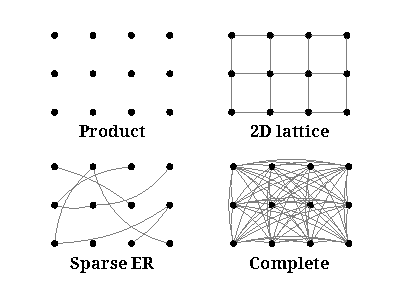
\includegraphics[width=\columnwidth]{ICML/lattice_illustration.pdf}}
    \caption{Illustration of the IQP architectures considered in this paper: product state (\cref{eg:product}), 2D lattice (\cref{eg:lattice}), sparse Erd\H os-R\'enyi graph (\cref{eg:sparse}), and complete graph (\cref{eg:complete}).}
    \label{pic:illustration}
  \end{center}
\end{figure}
%%%%%%%%%%%%%
\begin{example}[Product state]
\label{eg:product}
Consider the generator set that contains all the single-qubit generators, and nothing else. Then, fix a frequency $\vta \in \mathbb{F}_2^n \setminus \{\bm{0}\}$, the generators that anticommute with $X^\vta$ are exactly those whose support overlap with the support of $X^\vta$, i.e., $S^\vta=\{\bm{e}_k|a_k=1\}$, where $\bm{e}_k$ is the vector with $1$ on the $k$-th position. It is clear that all $\bm{e}_k$ are $\mathbb{F}_2$-linearly independent, so $r^\vta = \abs{a}$. Hence, low-weight Fourier frequencies with $\abs{\vta} \in \mathcal{O}(\log(n))$ will have polynomial decay variances, while high-weight frequencies with $\abs{\vta} \in \Theta(n)$ will have exponential decay variances. 
\end{example}

The model considered in \cref{eg:product} produces no entanglement and can only express product distributions. Even in such a simple model, characteristic function values at high-weight frequencies are already exponential decaying. This phenomenon is not unique to IQP-QCBM, but in fact an instance of global-observable-induced barren plateaus, which has already been studied in other quantum machine learning settings \cite{Cerezo21,rudolph24}. We move on with a more expressive generator set next.

\begin{example}[2D lattice]
\label{eg:lattice}
Let $G=(V,E)$ be a two-dimensional rectangular lattice graph on $n=\abs{V}$ qubits, where $(u,v)\in E$ are the edges of the lattice. Without loss of generality, we can consider $V = [n]$ for IQP circuits. Consider the generator set that contains all the single-qubit generators, and all the nearest-neighbor two-qubit generators, i.e, $\{\bm{e}_v : v\in V\} \cup \{\bm{e}_u+\bm{e}_v : (u,v)\in E\}$, where $\bm{e}_v\in \mathbb{F}_2^n$ is a basis vector consisting of all zero entries except at index $v$. Fix a Fourier frequency $\vta \in \mathbb{F}_2^n \setminus \{\bm{0}\}$, let
\begin{equation*}
    A:=\{v\in V: a_v=1\}
\end{equation*}
be the support of the observable $X^\vta$. For a single-qubit generator $\bm{e}_v$, we have that $\bm{e}_v\in S^\vta$ iff $v\in A$. For a two-qubit generator $\bm{e}_u+\bm{e}_v$, we have that $\vta \cdot (\bm{e}_u+\bm{e}_v)=a_u+a_v\ (\mathrm{mod}\ 2)$. Hence $\bm{e}_u+\bm{e}_v\in S^\vta$ iff exactly one of $\{u,v\}$ lies in $A$. Equivalently, the two qubit generators in $S^\vta$ are precisely the boundary edges of the cut $(A, V\setminus A)$, because 

Define the open neighborhood of $A$ by
\begin{equation}
B := \{u\in V: \exists v\in A  \text{ s.t. } (u,v)\in E\}.
\end{equation} and the closed neighborhood by $N[A] = A \cup B$. 
One can check that $r^\vta = \abs{N[A]}$, which depends not only on $\abs{\vta}$, but also on the topology of $A$. For the barren plateau analysis, it is convenient to simply bound the quantity $\abs{N[A]}$.
From above, we can use the fact that each $v\in A$ has at most $4$ distinct neighbors. Hence, we have
\begin{equation}
\abs{\vta}=\abs{A} \leq  r^\vta=\abs{N[A]} \leq \abs{A}+4\abs{A} = 5\abs{\vta}.
\end{equation}
Hence, low-weight Fourier frequencies with $\abs{\vta} \in \mathcal{O}(\log(n))$ will have polynomial decay variances, while high-weight frequencies with $\abs{\vta} \in \Theta(n)$ will have exponential decay variances.
\end{example}
%%%%%%%%%
The lattice architecture considered in \cref{eg:lattice} is already interesting because the model becomes universal for quantum computation under postselection \cite{Fujii17}. Consequently, by standard postselection-based hardness arguments, the existence of an efficient zero-error classical weak simulator would imply a collapse of the polynomial hierarchy to its third level. As a side remark, if no single-qubit generators are included, then the output distributions would be efficiently classically simulable \cite{Fujii17}.

\begin{example}[Sparse Erd\H os-R\'enyi graph]
\label{eg:sparse}
Consider the generator set that contains all the single-qubit generators, and a random subset of two-qubit generators $\{\bm{e}_u+\bm{e}_v\}$, where each pair $(i,j)$ is contained independently with probability $p=c \ln(n)/n$ for some constant $c=\Theta(1)$. Equivalently, let $G=(V,E)$ be an Erdos-Renyi graph with probability $c \ln(n)/n$. A two-qubit generator $\bm{e}_u+\bm{e}_v$ is included iff $(u,v)\in E$.

Just as in \cref{eg:lattice}, for a fixed Fourier frequency $\vta \in \mathbb{F}_2^n \setminus \{\bm{0}\}$, let $A$ be the support of the observable $X^\vta$, and denote the open and closed neighborhoods of $A$ by $B$ and $N[A]$ respectively. The equation $r^\vta = \abs{N[A]}$ also holds true here. For each  vertex $u\notin A$ the event $\{u\notin B\}$ occurs iff $u$ has no edge to any vertex in $A$.
\begin{equation}
\Pr[u\notin B] = (1-p)^{\abs{\vta}}
\end{equation}
Also, the events $\{u\in B\}$ are independent for each $u \notin A$.
Therefore, $\abs{B} \sim \mathrm{Binomial}(n-\abs{\vta},\,q)$, 
where $q = 1-(1-p)^{\abs{\vta}}$ and \begin{equation}\operatorname*{\mathbb{E}}_G[r^\vta] = \abs{\vta} + (n-\abs{\vta})q. \label{eq:sparse ra}
\end{equation}
Using that $(1-p)^\abs{\vta} = \exp(-p\abs{\vta} + \mathcal{O}(p^2\abs{\vta}))$, we can get that $q=p\abs{\vta} + \mathcal{O}((p\abs{\vta})^2)$ and $\operatorname*{\mathbb{E}}_G[r^\vta] \in \mathcal{O}(\log(n)^2)$ if $\abs{\vta} \in \mathcal{O}(\log(n))$, while $q = \Theta(1)$ and $\operatorname*{\mathbb{E}}_G[r^\vta] \in \Theta(n)$ if $\abs{\vta} \in \Theta(n)$. By Chernoff's bound, with high probability, for a single Erd\H os-R\'enyi graph, low-weight Fourier frequencies with $\abs{\vta} \in \Theta(1)$ will have polynomial decay, ($\abs{\vta} \in \mathcal{O}(\log(n))$ gives subexponential but not polynomial), while high-weight frequencies with $\abs{\vta} \in \Theta(n)$ will have exponential decay variances.
\end{example}

Note that the architecture considered in \cref{eg:sparse} is the same as the ``sparse IQP circuits'' proposed by \cite{Bremner17}, except that while we consider a continuous uniform distribution over $\vttheta$, they took $\vttheta$ uniformly from a discrete set. In particular, they showed that the existence of an efficient classical sampler that can output distributions
within small total variation distance to the true distributions of a constant fraction of instances from their ensemble of ``sparse IQP circuits'' would imply a collapse of the polynomial hierarchy
to its third level. \cite{Bremner17}

\begin{example}[Complete graph] \label{eg:complete} Consider the generator set that contains all the single-qubit generators and all the two-qubit generators. Fix a frequency $\vta \in \mathbb{F}_2^n \setminus \{\bm{0}\}$. Take any qubit that is in the support of $A$, call the supported single-qubit generator $\bm{e}_i$. Then, for all the qubits not in the support of $A$, the two-qubit generator $\bm{e}_i+\bm{e}_j \in S^\vta$. These two-qubit generators together with single-qubit generators supported by $A$ already form a basis. Therefore, for any frequency $\vta \in \mathbb{F}_2^n \setminus \{\bm{0}\}, r^\vta =n$, and the variances decay exponentially. 
\end{example}

Despite larger generator sets, the architectures in \cref{eg:lattice} and \cref{eg:sparse} still have polynomial decay variances for low-weight frequencies. Therefore, just like the product state architecture in \cref{eg:product}, by choosing a kernel with polynomial weights on the low-weight part of the spectrum, barren plateaus in the MMD can be avoided. However, for some even larger generator sets, e.g. that of \cref{eg:complete}, one will find that for any frequency $\vta \in \mathbb{F}_2^n \setminus \{\bm{0}\}$, the Fourier frequencies and their partial derivatives decay exponentially. Then no kernel can help avoid barren plateaus, as implied by \cref{prop:upper}. 

% \todo{1) Adrian's claim is correct
% 2) in general training to find the target in the general case is lost even with exp precision due to non-convexity of the landscapes (think non-local Z observable you may need to match) so shouod not be the goal
% 3) Indeed in the most general case for random initializations gradients may not exist
% 4) however many things can still work; first since any conjectural hard disrribution is still far in terms of MMD from some distributions IQPs can represent, it is easy to construct very special IQP architectures with few parameters (e.g. 1) which reach the (hard-wired) target distribution (which may be hard for a QC) starting from another distribution using MMD loss (the argument I had before)
% 5) another hting that can work is: we can use "weaker" IQP circuits which may sill be challenging for classical models and have signal : we (Kevin  ) proves this for local-lattice ZZs + zingle qubit operations which suffice for a sampling hardness result for zero error (via MBQC and post-selection arguments); further we can make it work with also non-local connections as long as the number of connectis is not too high. 
 
% For this reasons IQP based stuff may be useful in specialized applications as we envision.
%  }

\hw{I commented out this section. Instead, I think we should have a new section after ``Classical non-simulability and trainability'' showing the numerical results of training curves for the w/ and w/o BP cases.}
% \subsection{Absence of barren plateaus under Gaussian initialization} \label{subsec:gaussian}
% Here we apply \cref{thm: single symmetric} to the case where each parameter is i.i.d., and initialized by Gaussian distribution. We find that unlike uniform initialization, all characteristic function values, including those of high-weight frequencies, now have polynomial decay scalings. This finding is analogous to the results of \cite{zhang22}, which shows Gaussian initialization avoids barren plateaus for a variant of hardware-efficient circuit. This finding also supports the heuristic results on large gradient scalings in \cite{recioarmengol25}. However, we also note that under Gaussian initialization, the gates will be more closely concentrated around identity and hence more likely to be simulated classically. 
% \begin{theorem}[Characteristic function value partial derivative variance under Gaussian initialization]
% \label{thm:poly_lb_gaussian_mmd}
% Consider an $n$-qubit IQP-QCBM $U_\vttheta$ with generators $\{\vtsj\}$ of arbitrary architecture. Consider that the parameters $\vttheta$ are i.i.d. and Gaussian $\theta_j \sim\mathcal{N}(0,\gamma^2)$, with variance $\gamma^2 = c/D$ for arbitrary constant $c$. Fix $1\leq l \leq D$. For any frequency $\vta \in \mathbb{F}_2^n$, if $\in S^\vta$, then 
% \begin{equation}
% \operatorname*{Var}_{\vttheta} \left[ \frac{\partial C^\vta_\vttheta}{\partial \theta_\ell} \right] = \Omega\left(\mathrm{poly}(n^{-1})\right).
% \end{equation} 
% If $\vtsl \notin S^\vta$, then $\frac{\partial C^\vta_\vttheta}{\partial \theta_\ell}=0$.
% \end{theorem}

% \begin{remark}[Absence of barren plateaus under Gaussian initialization]
% Assume that $\exists \vta \in \mathbb{F}^2_n$ such that there exists a generator $\vtsl \in S^\vta$. This condition should be easily satisfied by most IQP architectures, including all previously considered examples. Then under \cref{ass:avgcase-target} and the further assumption that for that particular $\vta$, $\sigma_\vta^2 = \Omega\left(\mathrm{poly}(n^{-1})\right)$, the model will be partial-spectrum trainable and hence free of barren plateaus in the average case, i.e., 
% \begin{equation*}
% \operatorname*{\mathbb{E}}_p\left[\operatorname*{Var}_{\vttheta} \left[ \frac{\partial \mathcal{L}_\vttheta}{\partial \theta_\ell} \right]\right] = \Omega\left(\mathrm{poly}(n^{-1})\right)
% \end{equation*}
% \end{remark}

\subsection{Classical non-simulability and trainability}\label{subsec:non-simulability}
One of the most critical research questions regarding the quantum generative model is whether its output distribution can be efficiently simulated on a classical computer. In the literature~\cite{Bremner17}, proofs of non-simulability of the output distribution family of IQP requires that the family possess the so-called anti-concentration property.
%%%%%%%%%%%%%%%%%%%%
\begin{definition}[$L^2$ anti-concentration of family of discrete probability]
\label{def:anti-concentration}
Let $Q = \{q_\vttheta\}_\vttheta$ be a family of probability distributions in $\{0,1\}^n$. Assume a probability distribution of the parameter $\theta \sim P$, which makes $Q$ a random family/measure. We say $Q$ exhibits anti-concentration if the expected $L^2$-norm $\E\left(\norm{q_\vttheta}^2_2\right)\in\mathcal{O}(2^{-n})$ , i.e., there exists a constant $c>0$ such that: $\operatorname*{\mathbb{E}}_{\vttheta \sim P}\left[\sum_{x\in\{0,1\}^n} q_\vttheta(x)^2\right] \leq c/2^n$,
% \begin{equation}\label{eq:anti-concentration}
% \end{equation}
where the quantity $\sum_x q_\vttheta(x)^2$ is known as the collision probability.  
\end{definition}
Note that, \cref{def:anti-concentration} implies an alternative formulation of anti-concentration: there exist $\alpha>0,\beta>0$ such that $\forall x\in \{0,1\}^n, \;\Pr\left[q_\vttheta(x)\geq \alpha 2^{-n}\right]\ge \beta$,
which appears in sampling hardness arguments of IQP circuits~\cite{Bremner16, Bremner17}. To see this implication, we first observe that $\E_\vttheta(\sum_xq_\vttheta(x)) = 1\implies \E_\vttheta(q_\vttheta(x)) = 2^{-n}$ and $\E_\vttheta(q_\vttheta(x)^2) \le \E_\vttheta(\sum_xq_\vttheta(x)^2) \le c2^{-n}$, then we apply the Paley-Zygmund inequality to obtain $\Pr(q_\vttheta(x) \ge \alpha2^{-n}) \ge (1-\alpha)^2 2^{-n}/c$. Setting $\beta = (1-\alpha)^2/c$ completes the proof.

To investigate the anti-concentration of IQP-QCBM, it would be convenient to connect the condition in~\cref{def:anti-concentration} to the previous theorems in~\cref{subsec:uniform}. Since the Fourier/Hadamard transform is an $L^2$ isometry (the Parseval identity), we can achieve it automatically in the next lemma.
% Below, we focus on IQP-QCBMs under uniform initialization. In this setting, by parseval identity, we can alternatively express collision probabilities with Fourier frequencies. Then, using \cref{thm:uniform} allows us to equivalently write the definition of $L_2$ concentration using the quantities $r^\vta$. This serves as a bridge relating the absence or presence of barren plateau with anti-concentration.
%%%%%%%%%%%%%%%%%%%%
\begin{lemma}[$L^2$ anti-concentration of IQP-QCBM]
\label{lem:parseval} Let $Q = \{q_\vttheta\}_\vttheta$ be the random ensemble of output distributions of an IQP-QCBM with $\vttheta$ sampled u.a.r. in $[0,2\pi)^D$. Let $r^\vta = \dim\operatorname{span}_{\mathbb{F}_2}\left( S^{\vta} \right)$ defined as in~\cref{thm:uniform}. $Q$ is $L^2$ anti-concentrated iff. $\sum_{\vta\in\mathbb{F}_2^n}2^{-r^\vta} \in \mathcal{O}(1)\,.$
\end{lemma}
%%%%%%%%%%%%%%%%%%%%
\begin{proof}
    Let $C^\vta_\vttheta = \sum_{x\in \mathbb{F}_2^n} (-1)^{x\cdot \vta}q_\vtheta(x)$ be a characteristic function value.
    By the $L^2$ isometry of the Fourier transform, we have $\E_\vttheta\left(\sum_{\vta\in \mathbb{F}_2^n}(C^\vta_\vttheta)^2\right)=2^n\E_\vttheta\left(\norm{q_\vttheta}^2_2\right)\in\mathcal{O}(1)$. By~\cref{thm:uniform}, we have $\sum_{\vta\in \mathbb{F}_2^n}\E(C^\vta_\vttheta)^2=\sum_{\vta\in\mathbb{F}_2^n}2^{-r^\vta}.$
\end{proof}
%%%%%%%%%%%%%%%%%%%%
With the above lemma, we can easily check if the examples of IQP circuits in~\cref{subsec:uniform} have the anti-concentration property or not. \\
For~\cref{eg:product}, we verify the condition in~\cref{lem:parseval}:
%%%%%%%%%%%%%%%%%%%%
\begin{equation*}
\sum_{\vta \in \mathbb{F}_2^n}  2^{-r^\vta}=\sum_{k=0}^n \binom{n}{k}2^{-k}=\left(1+\frac12\right)^n=\left(\frac32\right)^n,
\end{equation*}
which means the model's output distribution is not anti-concentrated.\\
For~\cref{eg:lattice}, we verify the condition in \cref{lem:parseval}: 
\begin{equation*}
\sum_{k=0}^n \binom{n}{k}2^{-5k}=\left(\frac{33}{32}\right)^n
\leq
\sum_{\vta \in \mathbb{F}_2^n} 2^{-r^\vta}
\leq
\left(\frac32\right)^n,
\end{equation*}
which means the model's output distribution is not anticoncentrated. \\
In~\cref{eg:sparse}, the circuit connectivity $G$ graph is sampled from the Erd\H os-R\'enyi class, which we denote by $G\sim B(n,p)$. Note that the critical rank $r^{\vta}$ is a function of $G$. To emphasize it, we shall use the notation $r^{\vta}(G)$ here. We verify the condition in \cref{lem:parseval}: for any $c>2$, where $p=c\ln(n)/n$,
%%%%%%%%%%%%%%%%
\begin{equation}\label{eq:anti-concentration-sparse}
\operatorname*{\mathbb{E}}_{G\sim B(n,p)}\left(\sum_{\vta \in \mathbb{F}_2^n}  2^{-r^\vta(G)}\right)
= 2 + o(1)\,,
\end{equation} 
which means the model's output distribution is anti-concentrated. The complete derivation can be found in \cref{app:derivation-sparse}. In \cite{Bremner17}, they show anticoncentration in the discrete sparse IQP circuit ensemble. Our derivation is complementary. 
\\
For~\cref{eg:complete}, we verify the condition in \cref{lem:parseval}: \begin{equation}
\sum_{\vta \in \mathbb{F}_2^n} 2^{-r^\vta}
= 1+(2^n-1)2^{-n} = 2 - 2^{-n},
\end{equation}
%%%%%%%%%%%%%%%%
which means the model's output distribution is anti-concentrated. 
%%%%%%%%%%%%%%%%%%%%
% The expected collision probability $\operatorname*{\mathbb{E}}_{\vttheta} \left[Z\right]= \operatorname*{\mathbb{E}}_{\vttheta}\left[\sum_x q_\vttheta(x)^2\right]$ can be alternatively expressed as:
% \begin{equation}
% \operatorname*{\mathbb{E}}_{\vttheta}\big[Z\big] = 2^{-n}\sum_{\vta\in \mathbb{F}_2^n} \operatorname*{\mathbb{E}}_{\vttheta}\big[(C^\vta_\vttheta)^2\big]
% = 2^{-n}\sum_{\vta\in\mathbb{F}_2^n}2^{-r^\vta}.
% \end{equation}
% Then, the ensemble $\{q_\vttheta\}$ has $L_2$ anti-concentration iff there exists a constant $\alpha>0$ such that $\sum_{\vta\in\mathbb{F}_2^n}2^{-r^\vta} < \alpha $.
%%%%%%%%%%%%%%%%%%%%
\begin{theorem}[Existence of non-classically simulable and trainable IQP-QCBM]
\label{thm:ac_and_pst_exist}
There exists an IQP-QCBM with fixed generators, and the parameter $\vttheta$ follows an i.i.d. uniform distribution such that the ensemble of output distributions $\{q_\vttheta\}_\vttheta$ is hard to approximate classically up to additive error. Also, there exists a non-empty subset of Fourier frequencies $\mathcal{A} \subseteq \mathbb{F}_2^n$ such that this IQP-QCBM is $\mathcal{A}$-trainable with uniform initialization of $\vttheta$.
\end{theorem}
%%%%%%%%
\begin{proof}
    We consider the circuit connectivity graph $G$ generated by the sparse Erd\H os-R\'enyi model as in~\cref{eg:sparse}, i.e., for each pair $(i, j)$ of distinct qubits, we include a gate $\exp({i\theta Z_i\otimes Z_j})$ across those qubits with probability $c\log n/n$, for some fixed $c>2$. We also include all single-qubit Pauli-$Z$ rotations in the circuit. For this ensemble of IQP circuits, we have proven in~\cref{eq:anti-concentration-sparse} that its output distribution is anti-concentrated. Now, applying Markov inequality with~\cref{eq:anti-concentration-sparse}, we have the $\Pr\left(\sum_{\vta \in \mathbb{F}_2^n}  2^{-r^\vta(G)} \le \alpha\right) \ge 1 - 2/\alpha$, for a constant $\alpha >0$ (not a function of $n$), which means that if we choose a circuit from this random ensemble and keep the randomness of its parameter $\vttheta$ (uniform), we have a constant probability to obtain a single, parameterized IQP circuit with anti-concentration property.  \\
    \emph{Non-classically simulable}: Now, we apply Corollary 7 in~\cite{Bremner17}, saying that if $\{q_\vttheta\}_\vttheta$ is anti-concentrated (proven as above) and we assume there exists a classical polynomial-time algorithm $\mathcal{F}$ that, for each $U_\vtheta$, outputs a distribution approximately close to $q_\vttheta$ w.r.t. $\ell_1$-norm, then there is an $\text{FBPP}^{\text{NP}}$ algorithm (with access to $\mathcal{F}$) that approximates $q_\vttheta(x)$ for each $x\in\mathbb{F}_2^n$ up to a multiplicative error. As conjectured in~\cite{Bremner17}, approximating $q_\vttheta(x)$ with multiplicative error is \#P-hard, which leads to the collapse of the polynomial hierarchy if we assume such an algorithm $\mathcal{A}$ exists and the conjecture holds.\\
    \emph{Trainable}: as we showed in~\cref{eg:sparse}, for a fixed IQP connectivity graph sampled from Erd\H{o}s-R\'enyi, for Fourier frequency $|\vta|\in \Theta(1)$, $\operatorname{Var}(\partial C_\vttheta^\vta) \in \mathcal{O}(\mathrm{poly}(n^{-1}))$; for $|\vta|\in \mathcal{O}(\log(n))$, the variance decays subexponentially (but not polynomially); and for $|\vta|\in \Theta(n)$, the variance decays exponentially. Hence, it suffices to allocate the majority of the spectral distribution to the low-Hamming-weight frequencies, i.e., $\mathcal{A}=\{\vta\in\mathbb{F}_2^n \;\vert\; |\vta|\in \mathcal{O}(\log(n))\}$, to prevent the MMD loss gradient from exponential vanishing.
\end{proof}

\section{Discussion}
\label{sec:discussion}
Related to the topic of classical non-simulability and trainability, \citet{herbst25} claim that ``quantum models with sampling hardness rooted in anticoncentration will not be trainable''. We remark that their finding is not in contradiction with our results. The reason is that their argument relies on the concept of pseudo-independence, which is a strictly stronger condition than anti-concentration. A random measure $p$ is pseudo-independent if $p(x)=Y_x / (\sum_{j=1}^{2^n} Y_j)$ where $Y_j$ are identical and independent positive random variables. In fact, pseudo-independence implies anticoncentration, but the converse is false. They claim that output distributions of IQP circuits resemble pseudo-independent distributions (which is too strong as an assumption), and they prove that for a family of pseudo-independent distributions, MMD loss value vanishes exponentially w.r.t. the qubit number $n$ and hence conclude non-trainability. Their proof relies on the fact that pseudo-independence implies that the characteristic function values for all $\vta \neq \bm{0}$ are exponentially vanishing. In contrast, $L^2$ anti-concentration alone only constrains the collision probability, but still allows a small set of frequencies to remain polynomially visible. Our \cref{eg:sparse} exactly illustrates this subtle difference. We remark again that it is the anti-concentration needed in the proof of classical sampling hardness~\cite{Bremner16, Bremner17}, not pseudo-independence. 

Finally, we emphasize that training IQP-QCBM by minimizing $\MMD_k^2(p, q_\vttheta)$ for any choice of kernel $k$ does not imply that we can get a small total variation distance $\operatorname{TV}(p, q_\vttheta)$ since it is widely known that MMD is controlled by TV, but not vice versa. This limitation is purely classical information-theoretical, and not specific to IQP. It reflects the general fact that learning an arbitrary distribution on $\{0,1\}^n$ in total variation requires exponentially many samples in the worst case, since the space has $2^n-1$ degrees of freedom. 
% What methods, like MMD, can learn efficiently are restricted families. 










\section{Conclusions}
\label{sec:conclusion}
We study the trainability of IQP-QCBMs - a promising quantum generative model family, which is believed to have potential quantum advantage. In particular, we focus on investigating the scaling of the characteristic function of the output distribution of IQP-QCBM and of the MMD loss function.
% We give an architecture-level characterization of trainability for IQP-QCBMs under MMD. 
We first derive the closed-form variance expressions for the characteristic function values and the MMD and then identified the critical rank of the IQP model - the dimension of the space spanned (in $\mathbb{F}_2^n$) by the support of anti-commuting generators w.r.t. the observable, which determines the scaling of the loss gradient, and hence indicates the (non-)presence of BP. We precisely analyze whether barren plateaus occur in the MMD loss of four different IQP architectures under uniform initialization of the circuit's parameters, and demonstrate how BP can be mitigated by appropriate kernel selection.

We also show that trainability is not automatically incompatible with the classical non-simulability of IQP models. We show that for an IQP circuit whose connectivity is generated by a sparse Erd\H os-R\'enyi graph with $\mathcal{O}(n\log n)$ edges, its output distribution is hard to sample classically by applying the arguments from~\cite{Bremner17}. Also, this type of circuit is trainable: by allocating most of the spectral density to the low-Hamming-weight frequencies, we can avoid exponentially vanishing gradients of the MMD loss.

Lastly, we show that Gaussian initialization of the circuit's parameters leads to a polynomial decay in the variances of characteristic function values, even for high-weight frequencies, providing a potential way to broaden the set of trainable architectures in practice.



% \section*{Accessibility}

% Authors are kindly asked to make their submissions as accessible as possible
% for everyone including people with disabilities and sensory or neurological
% differences. Tips of how to achieve this and what to pay attention to will be
% provided on the conference website \url{http://icml.cc/}.

% \section*{Software and Data}

% If a paper is accepted, we strongly encourage the publication of software and
% data with the camera-ready version of the paper whenever appropriate. This can
% be done by including a URL in the camera-ready copy. However, \textbf{do not}
% include URLs that reveal your institution or identity in your submission for
% review. Instead, provide an anonymous URL or upload the material as
% ``Supplementary Material'' into the OpenReview reviewing system. Note that
% reviewers are not required to look at this material when writing their review.

% Acknowledgements should only appear in the accepted version.
% \section*{Acknowledgements}

% \textbf{Do not} include acknowledgements in the initial version of the paper
% submitted for blind review.

% If a paper is accepted, the final camera-ready version can (and usually should)
% include acknowledgements.  Such acknowledgements should be placed at the end of
% the section, in an unnumbered section that does not count towards the paper
% page limit. Typically, this will include thanks to reviewers who gave useful
% comments, to colleagues who contributed to the ideas, and to funding agencies
% and corporate sponsors that provided financial support.

\section*{Impact Statement}
This paper presents work whose goal is to advance the field of Machine
Learning. There are many potential societal consequences of our work, none
which we feel must be specifically highlighted here.


\bibliography{example_paper}
\bibliographystyle{icml2026}

%%%%%%%%%%%%%%%%%%%%%%%%%%%%%%%%%%%%%%%%%%%%%%%%%%%%%%%%%%%%%%%%%%%%%%%%%%%%%%%
%%%%%%%%%%%%%%%%%%%%%%%%%%%%%%%%%%%%%%%%%%%%%%%%%%%%%%%%%%%%%%%%%%%%%%%%%%%%%%%
% APPENDIX
%%%%%%%%%%%%%%%%%%%%%%%%%%%%%%%%%%%%%%%%%%%%%%%%%%%%%%%%%%%%%%%%%%%%%%%%%%%%%%%
%%%%%%%%%%%%%%%%%%%%%%%%%%%%%%%%%%%%%%%%%%%%%%%%%%%%%%%%%%%%%%%%%%%%%%%%%%%%%%%
\newpage
\appendix
\onecolumn
\section{Proof of Theorems}

\subsection{Proof of \cref{thm: single symmetric}}
Consider an $n$-qubit IQP-QCBM $U_\vttheta$ with generators $\{\vtsj\}$. Assume that the initialization satisfies \cref{ass:symm-iid-init}. For a fixed Fourier frequency $\vta \in \mathbb{F}_2^n \setminus \{\mathbf{0}\}$, define $S^{\vta} := \{ \vtsj \big| \vta \cdot \vtsj = 1 \}$, $
m^\vta := \abs{S^{\vta}}$. Let $
\Xi^\vta:= \{J\subseteq S^\vta:\ \sum_{j\in J}\vtsj=\mathbf 0 \}.$ Then, 
%%%%%%%%%
\begin{equation}
     \operatorname*{Var}_\vttheta \left[ C^\vta_\vttheta \right] = 
\left(\sum_{J\in \Xi^\vta} \mu^{|J|} \nu^{m^\vta-|J|}\right) - \kappa^{2m^\vta},
\end{equation}
%%%%%%%%%
where $\mu=\operatorname*{\mathbb{E}}_{\vttheta}[\sin^2(2\theta)]$, $\nu=\operatorname*{\mathbb{E}}_{\vttheta}[\cos^2(2\theta)]$, $\kappa=\operatorname*{\mathbb{E}}_{\vttheta}[\cos(2\theta)]$. Fix $1\leq l \leq D$. If $\vtsl \notin S^\vta$, then $ \frac{\partial C^\vta_\vttheta}{\partial \theta_\ell}=0$. If $\vtsl \in S^\vta$, then, 
%%%%%%%%%
\begin{align}
\operatorname*{Var}_\vttheta \left[ \frac{\partial C^\vta_\vttheta}{\partial \theta_\ell} \right]
&= 4\sum_{J\in \Xi^\vta}
\Bigl[
\bm{1}\{\ell\in J\}\,\mu^{|J|-1}\nu^{m^\vta-|J|+1} \notag
\\&+
\bm{1}\{\ell\notin J\}\,\mu^{|J|+1}\,\nu^{m^\vta-|J|-1}\Bigr].
\label{eq: symmetric variance}
\end{align}
%%%%%%%%%

\begin{proof}
Fix $\vta\neq \mathbf 0$ and abbreviate $S:=S^\vta$, $m:=m^\vta$. Start from the expression $C^\vta_\vttheta=\bra{+} U_\vttheta^\dagger X^{\vta}U_\vttheta\ket{+}
$. By recursively swapping the gates in $U_\vttheta$ with the observable $X^{\vta}$ and applying the commutation or anticommutation rule, one can derive the following:
\begin{align}
C^\vta_\vttheta
&= \bra{+}^{\otimes n} \prod_{\vtsj\in S^\vta} \exp(-2\theta_jZ^\vtsj) \ket{+}^{\otimes n} \\
&= \bra{+}^{\otimes n} \prod_{\vtsj\in S^\vta} (\cos(2\theta_j)I - i \sin(2\theta_j)Z^\vtsj) \ket{+}^{\otimes n}  \\
&= \sum_{J\in\Xi^\vta} R_J(\vttheta), \qquad R_J(\vttheta)=\eta_J 
\Bigl(\prod_{j\in J} \sin(2\theta_j)\Bigr)\Bigl(\prod_{j\in S\setminus J}\cos(2\theta_j)\Bigr),
\label{eq:C_subset_sum}
\end{align}
where $\eta_J \in \{-1,1\}$. The equation is a reformulation of equation 27 of \cite{recioarmengol25}. Note that $\forall J \in \Xi^\vta, \abs{J} = 0 \, (\text{mod 2})$, so no imaginary number $i$ appears. Also note that $\sin(\cdot)$ is an odd function, whose expectation vanishes for any initialization under \cref{ass:symm-iid-init}. We will use this property many times.

First, we derive the variance of the characteristic function values, $\operatorname*{Var}_\vttheta \left[ C^\vta_\vttheta \right] = \operatorname*{\mathbb{E}}_\vttheta \left[ (C^\vta_\vttheta)^2\right] - \left(\operatorname*{\mathbb{E}}_\vttheta \left[ C^\vta_\vttheta \right]\right)^2$. Regarding $\operatorname*{\mathbb{E}}_\vttheta \left[ C^\vta_\vttheta \right]$, except for the empty set $J = \emptyset$, all the other terms in the summation contain $\sin(2\theta_j)$ for some $j$ and hence vanish in expectation. Regarding $\operatorname*{\mathbb{E}}_\vttheta \left[ (C^\vta_\vttheta)^2\right]$, for the same reason, $\forall J \neq K$,  $\operatorname*{\mathbb{E}}_{\vttheta}[R_J(\vttheta)R_K(\vttheta)] = 0.$ Putting the remaining terms together gives the formula:
\begin{equation}
\label{eq: symmetric cost variance}
     \operatorname*{Var}_\vttheta \left[ C^\vta_\vttheta \right] = \left(\sum_{J \in \Xi^\vta} \operatorname*{\mathbb{E}}_{\vttheta}[\sin^2(2\theta)]^\abs{J} \operatorname*{\mathbb{E}}_{\vttheta}[\cos^2(2\theta)]^{m^\vta-\abs{J}}\right) - \operatorname*{\mathbb{E}}_{\vttheta}[\cos(2\theta)]^{2m^\vta}
\end{equation}
Then, we derive the variance of the partial derivatives. We differentiate \cref{eq:C_subset_sum} with respect to $\theta_\ell$. If $\vta \notin S^\vta$, then $\comm{Z^{\vts^\ell}}{X^\vta}=0$, so $C^\vta_\vttheta$ is independent of $\theta_\ell$, giving $\frac{\partial C^\vta_\vttheta}{\partial \theta_\ell}=0$. Now, if $\vtsl \in S^\vta$,

\begin{equation}
\frac{\partial C^\vta_\vttheta}{\partial\theta_\ell}
=
\sum_{J\in\Xi^\vta} T_J(\vttheta),
\end{equation}
where
\begin{equation}
T_J(\vttheta)
=
\begin{cases}
2 \eta_J\prod_{j\in J\setminus\{\ell\}}\sin(2\theta_j)\prod_{j\in (S\setminus J) \cup \{\ell\}}\cos(2\theta_j), & \ell\in J,\\
-2 \eta_J \prod_{j\in J\cup \{\ell \}}\sin(2\theta_j)\prod_{j\in (S\setminus J)\setminus\{\ell\}}\cos(2\theta_j), & \ell\notin J.
\end{cases}
\label{eq:TJ_def}
\end{equation}
For the same reason as before, $\operatorname*{\mathbb{E}}_{\vttheta}[T_J(\vttheta)T_K(\vttheta)] = 0 $ and  $\operatorname*{\mathbb{E}}_{\vttheta} \left[ \frac{\partial C^\vta_\vttheta}{\partial\theta_\ell}\right] = 0.$
Therefore,
\begin{equation}
\operatorname*{Var}_{\vttheta}\left[\frac{\partial C^\vta_\vttheta}{\partial\theta_\ell}\right]
=
\operatorname*{\mathbb{E}}_{\vttheta}\left[\left(\frac{\partial C^\vta_\vttheta}{\partial\theta_\ell}\right)^2\right]
=
\sum_{J\in \Xi^\vta}\operatorname*{\mathbb{E}}_{\vttheta}[T_J(\vttheta)^2],
\label{eq: symmetric derivative variance}
\end{equation}
Finally, by plugging in \cref{eq:TJ_def} gives the desired result.
\end{proof}

\subsection{Proof of \cref{prop:lower}}
Consider an $n$-qubit IQP-QCBM $U_\vttheta$ with generators $\{\vtsj\}$. Assume that the initialization satisfies \cref{ass:symm-iid-init}. Consider an arbitrary probability mass function of Fourier frequencies $\Lambda(\vta)$. Then, the MMD partial derivative yields the following decomposition.
\begin{equation}
\operatorname*{Var}_{\vttheta} \left[ \frac{\partial \mathcal{L}_\vttheta}{\partial \theta_\ell} \right] = 4 \operatorname*{\mathbb{E}}_{\vttheta} \biggl[ \sum_{\vta, \vtb} \Lambda(\vta) \Lambda(\vtb) \biggl( \nonumber - 2C^\vta_p C_\vttheta^\vtb \frac{\partial C_\vttheta^\vta}{\partial \theta_\ell} \frac{\partial C_\vttheta^\vtb}{\partial \theta_\ell} + 
 C^\vta_p C^\vtb_p \frac{\partial C_\vttheta^\vta}{\partial \theta_\ell} \frac{\partial C_\vttheta^\vtb}{\partial \theta_\ell} + C_\vttheta^\vta C_\vttheta^\vtb \frac{\partial C_\vttheta^\vta}{\partial \theta_\ell} \frac{\partial C_\vttheta^\vtb}{\partial \theta_\ell} \biggr) \biggr]
\end{equation}
Consider average-case target distributions drawn from a problem ensemble $\mathcal{P}$ that satisfies \cref{ass:avgcase-target}. Then, the quantity can be lower bounded as:
\begin{equation}
\operatorname*{\mathbb{E}}_{p\sim\mathcal{P}} \left[\operatorname*{Var}_{\vttheta} \left[ \frac{\partial \mathcal{L}_\vttheta}{\partial \theta_\ell} \right]\right] \geq
4 \sum_\vta G^2(\vta)\sigma_\vta^2\operatorname*{Var}_{\vttheta} \left[ \frac{\partial C^\vta_\vttheta}{\partial \theta_\ell} \right]
\end{equation}
where for a fixed $\vta$, $\sigma_\vta^2 =\operatorname*{\mathbb {E}}_{p}\left[(C_p^{\vta})^2\right]$ is the characteristic function value variance in the target distribution ensemble.

\begin{proof}
First, we expand the term inside the expectation $\operatorname*{\mathbb{E}}_p$ on L.H.S..
\begin{align}
    \operatorname*{Var}_{\vttheta} \left[ \frac{\partial \mathcal{L}_\vttheta}{\partial \theta_\ell} \right] &=    \operatorname*{Var}_{\vttheta} \left[ \frac{\partial }{\partial \theta_\ell}  \left(\sum_{\vta \in \mathbb{F}_2^n} \Lambda(\vta)\left(C^\vta_p - C^\vta_\vttheta \right)^2\right)\right]
\\ &= \operatorname*{Var}_{\vttheta} \left[-2 \sum_\vta \Lambda(\vta) \left(C^\vta_p - C^\vta_\vttheta \right) \frac{\partial C^\vta_\vttheta}{\partial \theta_\ell} \right] \\
&= 4 \sum_{\vta, \vtb} \Lambda(\vta) \Lambda(\vtb) \operatorname*{Cov}_{\vttheta}\left(\left(C^\vta_p - C^\vta_\vttheta\right) \frac{\partial C^\vta_\vttheta}{\partial \theta_\ell} , \left(C^\vtb_p - C^\vtb_\vttheta\right) \frac{\partial C^\vtb_\vttheta}{\partial \theta_\ell} \right) \\
&= 4 \sum_{\vta, \vtb} \Lambda(\vta) \Lambda(\vtb) \left(\operatorname*{\mathbb{E}}_{\vttheta} \left[ (C^\vta_p - C^\vta_\vttheta) \frac{\partial C^\vta_\vttheta}{\partial \theta_\ell} (C^\vtb_p - C^\vtb_\vttheta) \frac{\partial C^\vtb_\vttheta}{\partial \theta_\ell} \right] - \operatorname*{\mathbb{E}}_{\vttheta}\left[(C^\vta_p - C^\vta_\vttheta) \frac{\partial C^\vta_\vttheta}{\partial \theta_\ell} \right] \operatorname*{\mathbb{E}}_{\vttheta}\left[(C^\vtb_p - C^\vtb_\vttheta) \frac{\partial C^\vtb_\vttheta}{\partial \theta_\ell} \right] \right) \label{eq: one and two-copy vanish} \\
&= 4 \operatorname*{\mathbb{E}}_{\vttheta} \left[\sum_{\vta, \vtb} \Lambda(\vta) \Lambda(\vtb)  \left( C^\vta_p - C^\vta_\vttheta \right) \frac{\partial C^\vta_\vttheta}{\partial \theta_\ell} \left(C^\vtb_p - C^\vtb_\vttheta\right) \frac{\partial C^\vtb_\vttheta}{\partial \theta_\ell} \right] \\
&= 4 \operatorname*{\mathbb{E}}_{\vttheta} \left[ \sum_{\vta, \vtb} \Lambda(\vta) \Lambda(\vtb) \left( C^\vta_p C^\vtb_p \frac{\partial C_\vttheta^\vta}{\partial \theta_\ell} \frac{\partial C_\vttheta^\vtb}{\partial \theta_\ell} - C^\vta_p C_\vttheta^\vtb \frac{\partial C_\vttheta^\vta}{\partial \theta_\ell} \frac{\partial C_\vttheta^\vtb}{\partial \theta_\ell} - C^\vtb_p C_\vttheta^\vta \frac{\partial C_\vttheta^\vta}{\partial \theta_\ell} \frac{\partial C_\vttheta^\vtb}{\partial \theta_\ell} + C_\vttheta^\vta C_\vttheta^\vtb \frac{\partial C_\vttheta^\vta}{\partial \theta_\ell} \frac{\partial C_\vttheta^\vtb}{\partial \theta_\ell} \right)\right] \label{eq: two three four copies}
\end{align}
In the above derivation, many terms vanish. In specific, in \cref{eq: one and two-copy vanish}, all terms of the forms $\frac{\partial C_\vttheta^\vta}{\partial \theta_\ell} $ and $C^\vta_\vttheta\frac{\partial C_\vttheta^\vta}{\partial \theta_\ell}$ have zero expectation values. The reason is, these terms either vanish when $\vta \cdot\vtsl =0$, or are odd functions in $\theta_\ell$ when $\vta \cdot\vtsl =1$, the expectations of which vanish by the symmetry in the $\vttheta$ distribution.

To continue from \cref{eq: two three four copies}, we first identify the four-copy terms as square terms, i.e., 
\begin{equation}
    \operatorname*{\mathbb{E}}_{\vttheta} \left[ \sum_{\vta, \vtb} \Lambda(\vta) \Lambda(\vtb) C_\vttheta^\vta C_\vttheta^\vtb \frac{\partial C_\vttheta^\vta}{\partial \theta_\ell} \frac{\partial C_\vttheta^\vtb}{\partial \theta_\ell}\right] =\operatorname*{\mathbb{E}}_{\vttheta}\left[ \left(\sum_{\vta \in \mathbb{F}_2^n} \Lambda(\vta) C_\vttheta^\vta \frac{\partial C_\vttheta^\vta}{\partial \theta_\ell}\right)^2\right]
\end{equation}
which we can safely drop in the lower bound as non-negative terms. 

Then we can apply the ensemble average. Due to the mean-zero assumption on the characteristic function values, all the three-copy terms $C^\vta_p C_\vttheta^\vtb \frac{\partial C_\vttheta^\vta}{\partial \theta_\ell} \frac{\partial C_\vttheta^\vtb}{\partial \theta_\ell}$ vanish. Due to the uncorrelatedness assumptions on the characteristic function values, all the off-diagonal two copy terms $C^\vta_p C^\vtb_p \frac{\partial C_\vttheta^\vta}{\partial \theta_\ell} \frac{\partial C_\vttheta^\vtb}{\partial \theta_\ell}$ also vanish. Finally, we obtain the desired non-trivial lower bound for an average-case problem.
\begin{align}
 \operatorname*{\mathbb{E}}_p\left[\operatorname*{Var}_{\vttheta} \left[ \frac{\partial \mathcal{L}_\vttheta}{\partial \theta_\ell} \right]\right] &\geq 4 \operatorname*{\mathbb{E}}_{\vttheta}  \left[ \sum_{\vta \in \mathbb{F}_2^n} \Lambda(\vta)^2 (C^\vta_p)^2 \left(\frac{\partial C_\vttheta^\vta}{\partial \theta_\ell}\right)^2 \right] \\
 &= 4 \sum_a\Lambda(\vta)^2\sigma_\vta^2\operatorname*{Var}_{\vttheta} \left[ \frac{\partial C^\vta_\vttheta}{\partial \theta_\ell} \right] 
\end{align}
\end{proof}

\subsection{Proof of \cref{prop:upper}}
Consider an $n$-qubit IQP-QCBM $U_\vttheta$ with generators $\{\vtsj\}$. Consider an arbitrary initialization scheme. Consider an arbitrary probability mass function of Fourier frequencies $\Lambda(\vta)$. The MMD partial derivative variance can be upper bounded as:
\begin{equation}
    \operatorname*{Var}_{\vttheta} \left[ \frac{\partial \mathcal{L}_\vttheta}{\partial \theta_\ell} \right] \leq 16 \sum_\vta \Lambda(\vta)\left[  \operatorname*{Var}_{\vttheta} \left[ \frac{\partial C^\vta_\vttheta}{\partial \theta_\ell} \right]\right]
\end{equation}
\begin{proof}
\begin{align}
\operatorname*{Var}_{\vttheta} \left[ \frac{\partial \mathcal{L}_\vttheta}{\partial \theta_\ell} \right] &\leq \operatorname*{\mathbb{E}}_{\vttheta} \left[ \left(\frac{\partial \mathcal{L}_\vttheta}{\partial \theta_\ell} \right)^2 \right] \\
&= 4\operatorname*{\mathbb{E}}_{\vttheta} \left[  \operatorname*{\mathbb{E}}_{\vta}\left[\left( C^\vta_p - C^\vta_\vttheta \right) \frac{\partial C^\vta_\vttheta}{\partial \theta_\ell} \right]^2  \right] \label{eq: upper line 2}\\
&\leq 4\operatorname*{\mathbb{E}}_{\vttheta} \left[  \operatorname*{\mathbb{E}}_{\vta}\left[\left( C^\vta_p - C^\vta_\vttheta \right)^2 \right] \operatorname*{\mathbb{E}}_{\vta}\left[\left(\frac{\partial C^\vta_\vttheta}{\partial \theta_\ell} \right)^2\right]\right] \label{eq: upper line 3}\\
&\leq 4\operatorname*{\mathbb{E}}_{\vttheta} \left[  4 \operatorname*{\mathbb{E}}_{\vta}\left[\left(\frac{\partial C^\vta_\vttheta}{\partial \theta_\ell} \right)^2\right]\right] \label{eq: upper line 4}\\
&= 16 \sum_\vta \Lambda(\vta)\left[  \operatorname*{Var}_{\vttheta} \left[ \frac{\partial C^\vta_\vttheta}{\partial \theta_\ell} \right]\right] \label{eq: upper line 5}
\end{align}
From \cref{eq: upper line 2} to \cref{eq: upper line 3}, we use the Cauchy-Schwarz inequality. From \cref{eq: upper line 3} to \cref{eq: upper line 4}, we use the bound that for a fixed $\vta$, $(C^\vta_p - C^\vta_\vttheta)^2 \leq 4$. From \cref{eq: upper line 4} to \cref{eq: upper line 5}, we exchange the order of expectations over $\vta$ and $\vttheta$, and use the fact that $\operatorname*{\mathbb{E}}_{\vttheta}\left[\partial C^\vta_\vttheta / \partial \theta_\ell\right] = 0$.
\end{proof}

\subsection{Proof of \cref{thm:uniform}}
Consider an $n$-qubit IQP-QCBM $U_\vttheta$ with generators $\{\vtsj\}$. Consider that the parameters are initialized from i.i.d. uniform distribution $\theta_j \sim\mathcal{U}[0,2\pi)$. For a fixed Fourier frequency $\vta \in \mathbb{F}_2^n \setminus \{\mathbf{0}\}$, define $S^{\vta} := \{ \vtsj \big| \vta \cdot \vtsj = 1 \}$ and define the critical rank $r^\vta := \dim \operatorname{span}_{\mathbb{F}_2}\left( S^{\vta} \right)$, which is the number of $\mathbb{F}_2$-linearly independent generators. Then, \begin{equation}
\operatorname*{Var}_{\vttheta} \left[ C^\vta_\vttheta\right] = 2^{-r^\vta}. 
\end{equation} Fix $1\leq l \leq D$. If $\vtsl \notin S^\vta$, then $ \frac{\partial C^\vta_\vttheta}{\partial \theta_\ell}=0$. If $\vtsl \in S^\vta$, then
\begin{equation}
\operatorname*{Var}_{\vttheta} \left[ \frac{\partial C^\vta_\vttheta}{\partial \theta_\ell} \right] = 2^{\,2-r^\vta}. \end{equation}
\begin{proof}
Since the i.i.d. uniform initialization satisfies \cref{ass:symm-iid-init}, \cref{eq: symmetric cost variance} and \cref{eq: symmetric derivative variance} from \cref{thm: single symmetric} apply here, and we adopt the same notations in this proof. In the case of uniform distribution, $\mu = \nu = 1/2$ and $\kappa = 0$. Plugging in these values gives, \begin{equation}
    \operatorname*{Var}_\vttheta \left[ C^\vta_\vttheta \right] = 2^{-m^\vta} \abs{\Xi^\vta} , \qquad \operatorname*{Var}_{\vttheta}\left[\frac{\partial C^\vta_\vttheta}{\partial\theta_\ell}\right]
= 2^{2-m^\vta} \abs{\Xi^\vta} 
\end{equation}
Note that $\Xi^\vta$ is isomorphic to the set $\{\vtx \in \mathbb{F}_2^n | A \vtx = \bm{0}\}$, where $A$ is the matrix whose columns are the elements of $S^\vta$. In other words, $\Xi^\vta$ is the kernel of $A$ and hence $\abs{\Xi^\vta} = 2^{m^\vta-r^\vta}$ by rank-nullity theorem. This completes the proof.
\end{proof}

\subsection{Proof of \cref{thm:poly_lb_gaussian_mmd}}
Consider an $n$-qubit IQP-QCBM $U_\vttheta$ with generators $\{\vtsj\}$ of arbitrary architecture. Consider that the parameters $\vttheta$ are i.i.d. and Gaussian $\theta_j \sim\mathcal{N}(0,\gamma^2)$, with variance $\gamma^2 = c/D$ for arbitrary constant $c$. Fix $1\leq l \leq D$. For any frequency $\vta \in \mathbb{F}_2^n$, if $\in S^\vta$, then 
\begin{equation}
\operatorname*{Var}_{\vttheta} \left[ \frac{\partial C^\vta_\vttheta}{\partial \theta_\ell} \right] = \Omega\left(\mathrm{poly}(n^{-1})\right).
\end{equation} 
If $\vtsl \notin S^\vta$, then $\frac{\partial C^\vta_\vttheta}{\partial \theta_\ell}=0$.
\begin{proof}
We assume that $\vta \in \vtsl$ and continue from \cref{eq: symmetric variance} of \cref{thm: single symmetric},
\begin{equation}
\operatorname*{Var}_{\vttheta}\!\left(\frac{\partial C_\vttheta^\vta}{\partial\theta_\ell}\right)
=
4\sum_{J\in \Omega^\vta}
\left[
\bm{1}\{\ell\in J\}\,\mu^{|J|-1}\nu^{m^\vta-|J|+1}
+
\bm{1}\{\ell\notin J\}\,\mu^{|J|+1}\,\nu^{m^\vta-|J|-1}
\right],
\label{eq:single_var_exact_c}
\end{equation}
We identify \begin{equation}
    \mu:=\operatorname*{\mathbb{E}}_{\theta\sim\mathcal N(0,\gamma^2)}[\sin^2(2\theta)]
=\frac{1-e^{-8\gamma^2}}{2},
\qquad
\nu:=\operatorname*{\mathbb{E}}_{\theta\sim\mathcal N(0,\gamma^2)}[\cos^2(2\theta)]
=\frac{1+e^{-8\gamma^2}}{2}
\end{equation} 
Note that every term in the summation is nonnegative. For the proof it suffices to keep the term $J= \emptyset$ and drop other terms, which gives
\begin{align}
\operatorname*{Var}_{\vttheta}\!\left(\frac{\partial C_\vttheta^\vta}{\partial\theta_\ell}\right) & \geq 
4\mu\,\nu^{m^\vta-1} \\
& \geq  4\mu\,\nu^{D-1} 
\label{eq:single_var_lb_c}
\end{align}
By Taylor expansion, we can derive that $\mu = 4c/D + o(1/D)$ and $\nu^{D-1} = e^{-4c} + o(1)$. Therefore, $4\mu \nu^{D-1} =\Theta(1/D)$, which completes the proof.
\end{proof}

\newpage 

\section{Derivation details}
\subsection{Complete derivation of anti-concentration in the sparse Erdos-Renyi graph (\cref{eg:sparse})}
\label{app:derivation-sparse}
Based on \cref{eq:sparse ra}, we 
get that 
\begin{equation}
\operatorname*{\mathbb{E}}_G\big[2^{-r^\vta}\big]
=
2^{-\abs{\vta}}\mathbb{E}\big[2^{-|B|}\big]
=
2^{-\abs{\vta}}\left(1-\frac{q}{2}\right)^{n-\abs{\vta}},
\end{equation} where the last equality is obtained by the formula of generating function of the binomial random variable $\abs{B}$. Then,
\begin{equation}
\operatorname*{\mathbb{E}}_G\left[\sum_{\vta \in \mathbb{F}_2^n}  2^{-r^\vta}\right]
=
\sum_{k=0}^n \omega_k\left(1+\lambda^k\right)^{n-k}, \qquad \omega_k=\binom{n}{k}2^{-n}, \qquad \lambda=1-p.
\end{equation}
We can rewrite this as three parts:
\begin{align}
\operatorname*{\mathbb{E}}_G\left[\sum_{\vta \in \mathbb{F}_2^n}  2^{-r^\vta}\right] &= \omega_0 \cdot 2^n + \sum_{k=1}^n \omega_k + \sum_{k=1}^n \omega_k \left((1+\lambda^k)^{n-k} - 1 \right) \\
&=1+(1-2^{-n})+R_n
\end{align}
where $R_n:=\sum_{k=1}^n w_k\Bigl[(1+\lambda^k)^{n-k}-1\Bigr].$
We split $R_n=R_{1,n}+R_{\ge2,n}$ with
\begin{equation}
R_{1,n}=w_1\bigl[(1+\lambda)^{n-1}-1\bigr]
= n2^{-n}\bigl[(2-p)^{n-1}-1\bigr].
\end{equation}

Define the shorthand
\begin{equation}
T_n:=n2^{-n}(2-p)^{n-1}=\frac{n}{2-p}\Bigl(1-\frac{p}{2}\Bigr)^n = \frac{n}{2-p} \exp\left(-\frac{np}{2} + \mathcal{O}(np^2)\right). \label{eq:Tn}
\end{equation}
With $p=c \ln(n)/n$, we have \begin{equation}
T_n = (1/2 + o(1))n^{1-c/2}
\end{equation}

\noindent
Moreover,
\begin{equation}\label{eq:R1-asymp}
R_{1,n}=T_n+o(T_n).
\end{equation}

Now it is left to deal with $R_{\ge2,n}$. For each $k$, we can separate the term inside as a linear part and a remainder part. \begin{equation}
(1+\lambda^k)^{n-k} - 1 = (n-k)\lambda^k + \Delta(k,n)
\end{equation}
Then \begin{equation}
    R_{\ge2,n} = \sum_{k\geq 2} \omega_k (n-k)\lambda^k + \sum_{k\geq 2} \omega_k\Delta(k,n)
\end{equation}
For the summation over linear parts, using that $(n-k)\binom{n}{k} = n \binom{n-1}{k}$, we get 
\begin{equation}
    \sum_{k=0} \omega_k (n-k)\lambda^k = n2^{-n} \sum_{k=0}^{n-1} \binom{n-1}{k} \lambda^k = n2^{-n}(2-p)^{n-1} = T_n
\end{equation}
Removing the terms for $k=0$ and $k=1$ gives
\begin{equation}
    \sum_{k\geq 2} \omega_k (n-k)\lambda^k = T_n + o(T_n)
\end{equation}
When $c>2$, $T_n = o(1)$, and since the summation over remainders is dominated by the summation over linear parts. Putting everything together gives
\begin{equation}
    \operatorname*{\mathbb{E}}_G\left[\sum_{\vta \in \mathbb{F}_2^n}  2^{-r^\vta}\right] = 2 + o(1)
\end{equation}
\end{document}

% This document was modified from the file originally made available by
% Pat Langley and Andrea Danyluk for ICML-2K. This version was created
% by Iain Murray in 2018, and modified by Alexandre Bouchard in
% 2019 and 2021 and by Csaba Szepesvari, Gang Niu and Sivan Sabato in 2022.
% Modified again in 2023 and 2024 by Sivan Sabato and Jonathan Scarlett.
% Previous contributors include Dan Roy, Lise Getoor and Tobias
% Scheffer, which was slightly modified from the 2010 version by
% Thorsten Joachims & Johannes Fuernkranz, slightly modified from the
% 2009 version by Kiri Wagstaff and Sam Roweis's 2008 version, which is
% slightly modified from Prasad Tadepalli's 2007 version which is a
% lightly changed version of the previous year's version by Andrew
% Moore, which was in turn edited from those of Kristian Kersting and
% Codrina Lauth. Alex Smola contributed to the algorithmic style files.
